% ****** Start of file apssamp.tex ******
%
%   This file is part of the APS files in the REVTeX 4.1 distribution.
%   Version 4.1r of REVTeX, August 2010
%
%   Copyright (c) 2009, 2010 The American Physical Society.
%
%   See the REVTeX 4 README file for restrictions and more information.
%
% TeX'ing this file requires that you have AMS-LaTeX 2.0 installed
% as well as the rest of the prerequisites for REVTeX 4.1
%
% See the REVTeX 4 README file
% It also requires running BibTeX. The commands are as follows:
%
%  1)  latex apssamp.tex
%  2)  bibtex apssamp
%  3)  latex apssamp.tex
%  4)  latex apssamp.tex
%
\documentclass[%
 reprint,
%superscriptaddress,
%groupedaddress,
%unsortedaddress,
%runinaddress,
%frontmatterverbose, 
%preprint,
%showpacs,preprintnumbers,
%nofootinbib,
%nobibnotes,
%bibnotes,
 amsmath,amssymb,
 aps,
%pra,
%prb,
%rmp,
%prstab,
%prstper,
%floatfix,
]{revtex4-1}

\usepackage{graphicx}% Include figure files
\usepackage{dcolumn}% Align table columns on decimal point
\usepackage{bm}% bold math
%\usepackage{hyperref}% add hypertext capabilities
%\usepackage[mathlines]{lineno}% Enable numbering of text and display math
%\linenumbers\relax % Commence numbering lines

%\usepackage[showframe,%Uncomment any one of the following lines to test 
%%scale=0.7, marginratio={1:1, 2:3}, ignoreall,% default settings
%%text={7in,10in},centering,
%%margin=1.5in,
%%total={6.5in,8.75in}, top=1.2in, left=0.9in, includefoot,
%%height=10in,a5paper,hmargin={3cm,0.8in},
%]{geometry}
\usepackage{ctex}
\usepackage{amsmath}
\usepackage{siunitx}


\begin{document}

\preprint{APS/123-QED}

\title{相对论性重离子对撞实验与STAR探测器介绍}% Force line breaks with \\
\author{钱思天}
 \email{stqian@pku.edu.cn}
\affiliation{%
北京大学~物理学院~技术物理系
}%


\date{\today}% It is always \today, today,
             %  but any date may be explicitly specified

\begin{abstract}
相对论性重离子碰撞是研究量子色动力学(QCD)特别是夸克胶子等离子体(QGP)的重要甚至是目前唯一的实验手段。利用相对论性重离子碰撞实验,可以对QCD参数给出进一步的限制。坐落于美国布鲁克海文国家实验室(BNL)的相对论性重离子对撞机(RHIC)及其上的STAR探测器,是研究相对论性重离子碰撞的重要实验。本文将通过对相对论性重离子碰撞和STAR探测器的介绍,尝试给读者带来一些对高能核物理实验的基本认识。
\end{abstract}

\pacs{Valid PACS appear here}% PACS, the Physics and Astronomy
                             % Classification Scheme.
%\keywords{Suggested keywords}%Use showkeys class option if keyword
                              %display desired
\maketitle

%\tableofcontents

\section{\label{sec:bgd}背景介绍}



\subsection{\label{sec:Phybg}物理背景}

相对论性重离子碰撞是研究量子色动力学特别是夸克胶子等离子体(QGP)的重要甚至是目前唯一的实验手段\cite{Ruan:2005hy}\cite{Dong:2005iq}。由于QCD的跑动耦合常数(如图\ref{fig:Running})带来的渐进自由效应,QGP的性质无法通过第一性原理微扰计算得到,格点数值计算也因为计算资源的限制举步维艰,使得人类目前只能从一些唯象角度进行建模\cite{Qiu:2013wca}。
\begin{figure}[htbp]
    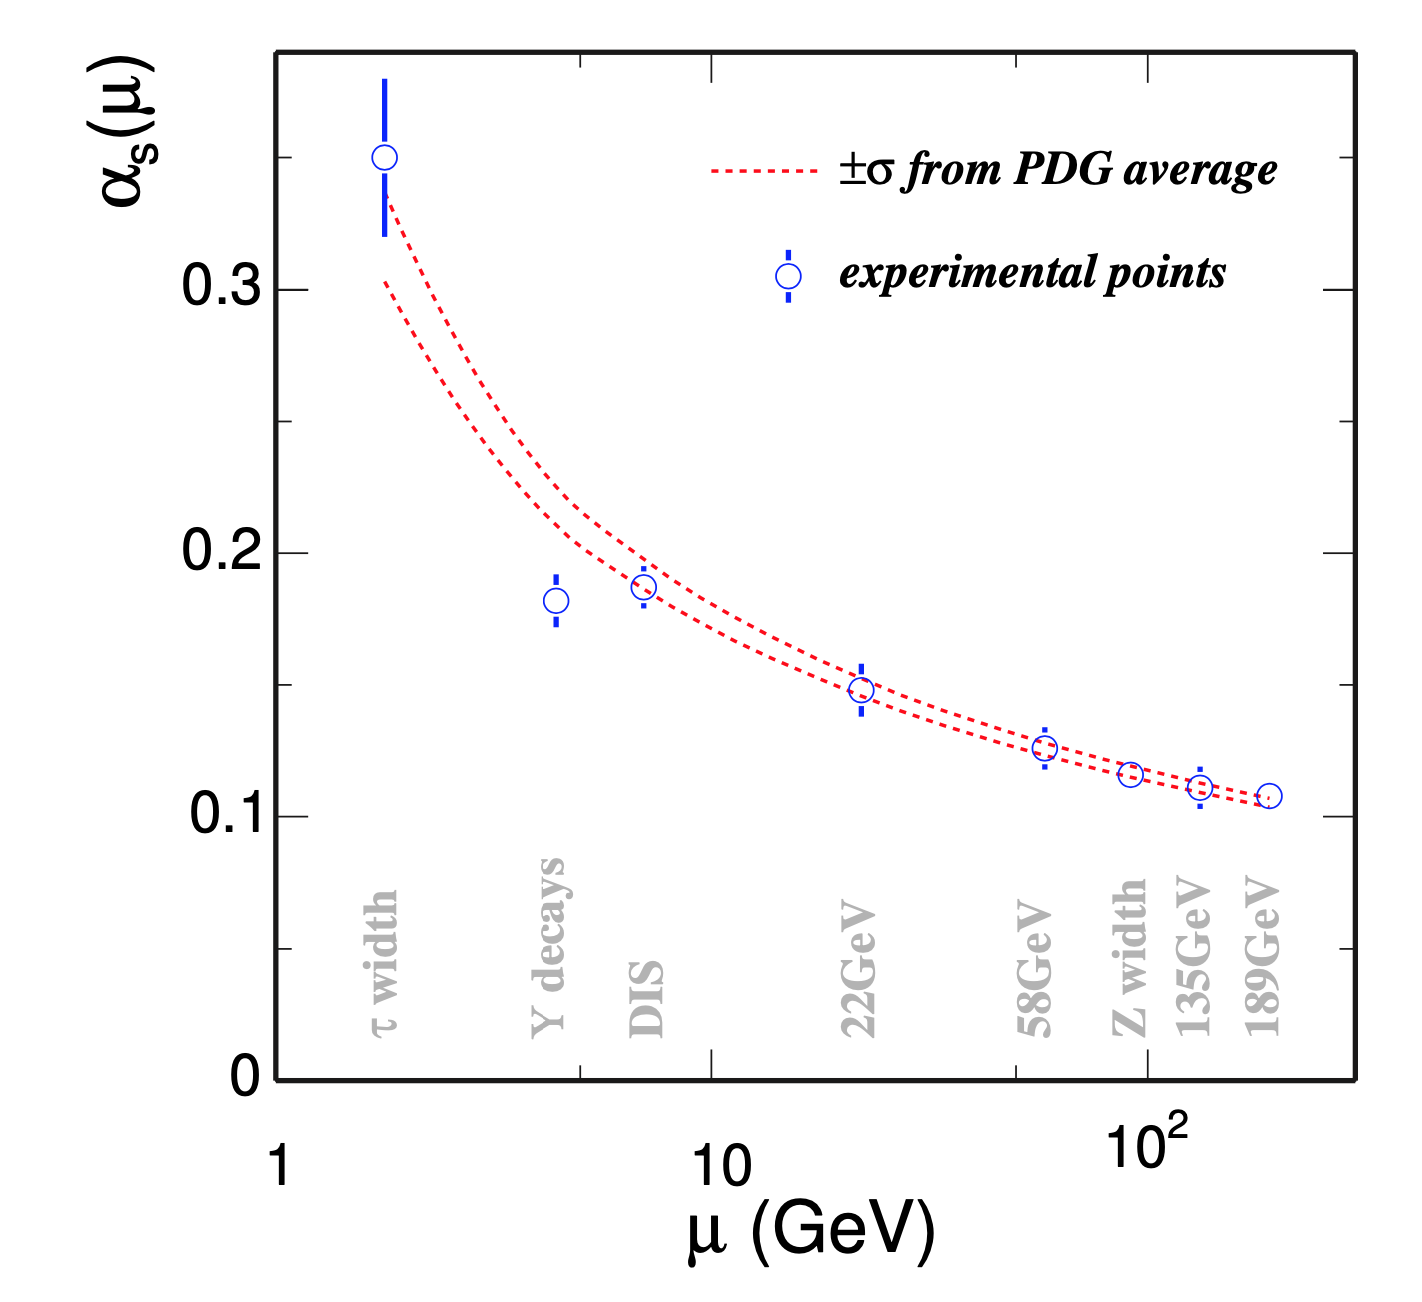
\includegraphics[width = 0.4\textwidth]{Plots/Running.png}
    \caption{\label{fig:Running}QCD的跑动耦合常数}
\end{figure}
\subsubsection{\label{sec:QGP}夸克胶子等离子体(QGP)}
在量子色动力学的观点被广为接受之后,夸克胶子等离子体(Quark Gluon Plasma)作为一种物理实体\ref{fig:QCD}的概念被自然而然的提了出来。
\begin{figure}[htbp]
    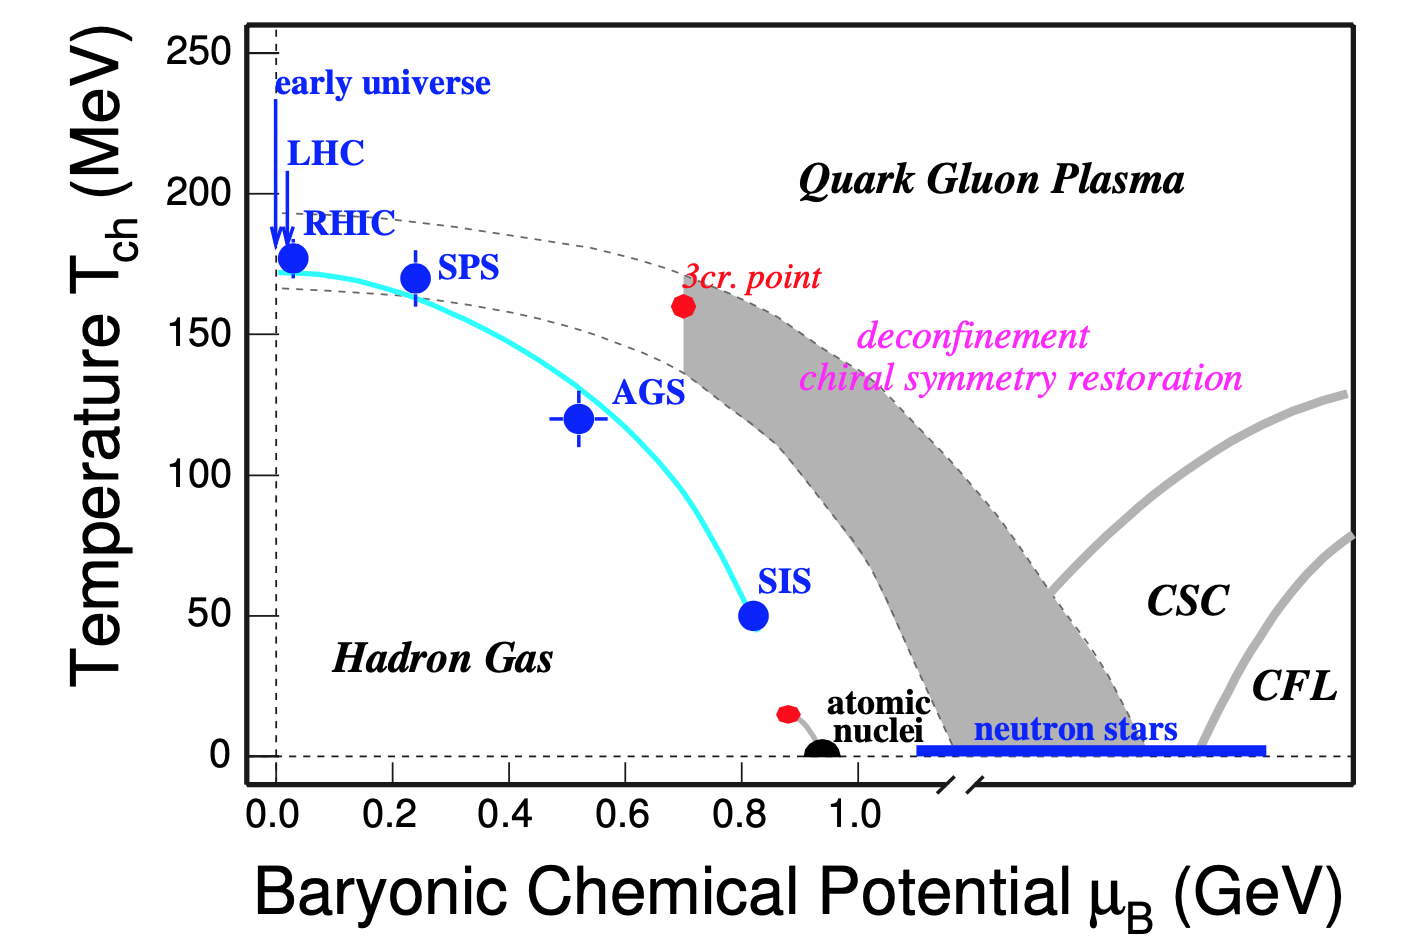
\includegraphics[width = 0.4\textwidth]{Plots/QCDPD.png}
    \caption{\label{fig:QCD}QCD相图,QGP位于高温高密区域}
\end{figure}
但是,当QGP第一次被提及时,它的性质被认为和气体相似\footnote{但又并非是强子气体(Hadron Resonance Gas)。},即夸克、胶子之间的相互作用很弱。在没有相关实验数据之前,这种观点一直占据主导地位。但当第一次对相对论性重离子碰撞的中心快度区域进行观测后,人们发现了诸如在末态强子谱中存在角度关联等实验证据,进而意识到QGP中的夸克胶子间的相互作用强于预期\cite{Adams:2005dq}。
\subsubsection{\label{sec:HIC}相对论性重离子碰撞}
由于跑动耦合常数带来的渐近自由效应,想要产生QGP,就不得不要求系统处在极端高温高密的环境下。相比于传统的质子与电子对撞机,重离子碰撞有着的初始能量密度随着原子数增加呈幂指数律增加的同时对于碰撞能量仅仅是幂次增加这一优势,特别适用于产生QGP信号并进行寻找。而在世界上的这些相对论性重离子碰撞实验中比较重要与引人注目的,当数位于美国纽约长岛布鲁克海文国家实验室(BNL)的相对论性重离子对撞机(RHIC)和其上的相关实验\cite{Adams:2005dq}。
\subsection{\label{sec:ExpBG}实验背景}
\subsubsection{\label{sec:RHICBg}RHIC背景简述}
作为美国高能物理实验重镇,BNL有着悠久的加速器传统,例如中国人耳熟能详的杨振宁与李政道的弱相互作用中宇称不守恒的理论工作,出发点是他们在BNL工作期间为了解释COSMOTRON加速器上所做粒子衰变实验的结果,又比如丁肇中发现$J/\psi$粒子,也是在BNL的AGS加速器上完成的。值得一提的是,AGS加速器的设计之初便考虑了对重离子的加速,后来,他也作为了RHIC的初级加速装置被保留了下来\footnote{类似的“传承”还有SPS与LHC。}。

\subsubsection{\label{sec:RHICSpec}RHIC技术参数简介}
下面对RHIC的技术参数做进一步的说明,其正式完成于1999年,是当时世界上加速能量最高的重离子对撞装置,可以达到$100\si{GeV/u}$。表\ref{tab:RhicSpec}中给出了RHIC的一些重要物理参数\cite{Ruan:2005hy}\cite{Dong:2005iq}:
\begin{table}[htbp]
    \centering
    \caption{\label{tab:RhicSpec}RHIC的一些重要技术参数}
    \begin{ruledtabular}
    \begin{tabular}{cc}
    技术指标&值  \\
    \colrule
    Top Au+Au $\sqrt{s_{NN}}$&$200 \si{GeV}$ \\
    Top p+p $\sqrt{s_{NN}}$&$500 \si{GeV}$ \\
    Ave. luminosity (Au+Au) & $\sim 2\times10^{26}\si{\per \square cm \per s}$ \\
    Ave. luminosity (p+p) & $\sim 4\times10^{30}\si{\per \square cm \per s}$ \\ 
    Bunches per ring & 6 \\
    Ions per bunch (Au) & $10^9$ \\
    Ions per bunch (proton) & $10^{11}$ \\
    Beam lifetime (store length) & 10 hours\\
    RHIC circumference & 3.8 km
    \end{tabular}
    \end{ruledtabular}
\end{table}

作为大型加速器,RHIC上同时进行的实验并不只一处,同时,正如前文所述,RHIC的组成部分也并不单一。下图\ref{fig:RHIC}就展示了RHIC的一些大略的实验结构。
\begin{figure}[htbp]
    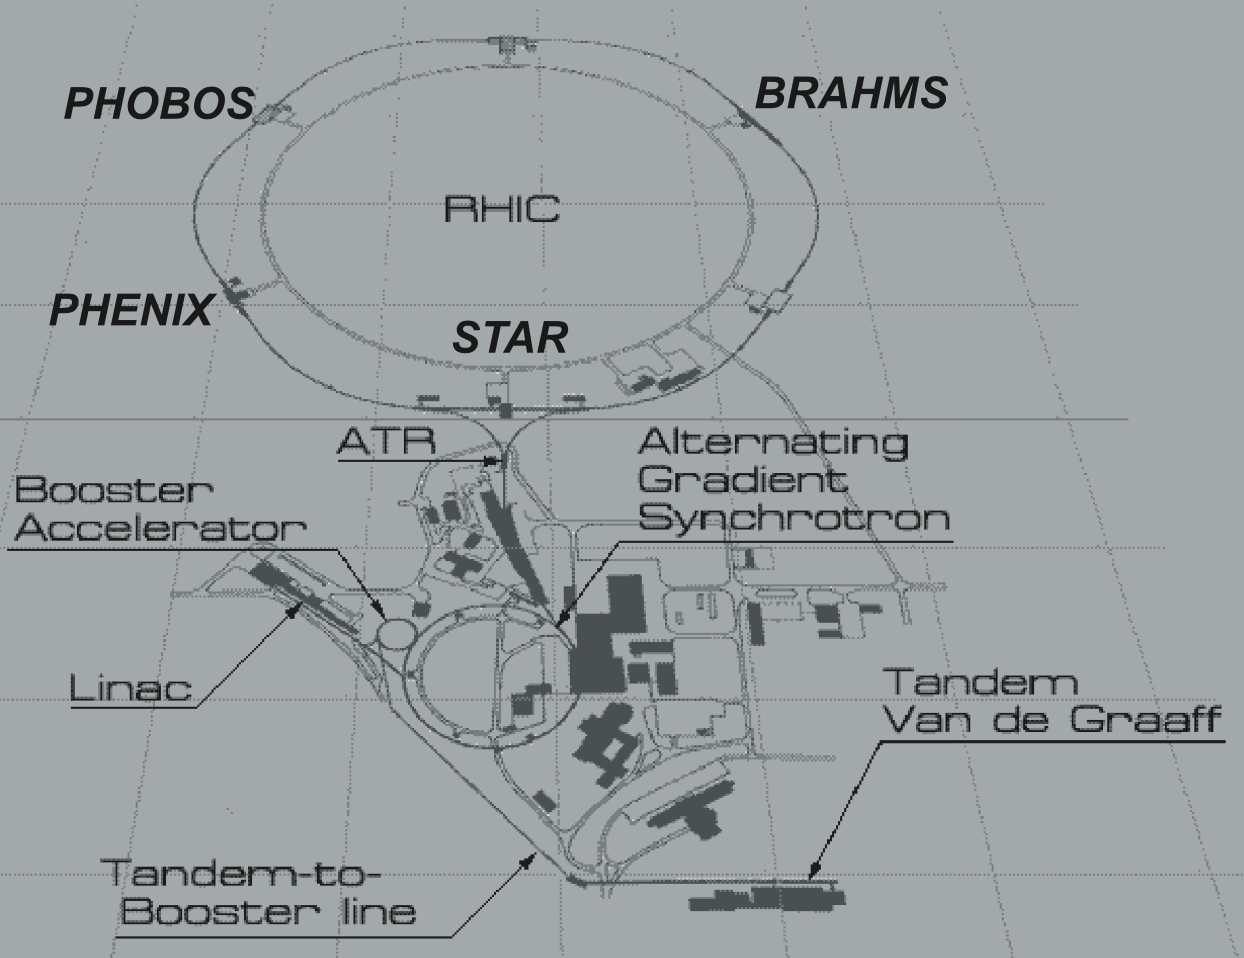
\includegraphics[width=0.4\textwidth]{Plots/RHIC.png}
    \caption{\label{fig:RHIC}RHIC的平面图}
\end{figure}
其中,加粗的黑色字体是RHIC上主要运行的四个探测器及实验。而靠下方的部分则是RHIC的各级加速装置。虽然最终都会在环上进行回旋加速,但是和来自于直线加速器(Linac)的质子不同,重离子的各级加速相对较为复杂:产生于脉冲溅射离子源(Pulsed Sputter Ion Source)串列中的金原子束被前后范德格拉夫(Tandem Van de Graaff)加速器加速然后通过两个金箔来剥离掉部分电子,得到约$1\si{MeV/u}$,带32个单位正电荷的金离子束。这些离子束会通过增压器(Booster)加速到能量为$95\si{MeV/u}$并进一步剥离电子到电荷为+77态然后注入到AGS,在加速到$8.86\si{GeV/u}$每核子并进一步剥离掉剩下的轨道电子后才会由AGS-To-RHIC(ATR)转移线注入RHIC环。

RHIC的物理目标就是为了达到产生QGP的相变条件,因此,在RHIC运行之后,人们便通过其上进行的PHENIX实验进行了验证。通过对实验数据的分析,人们发现RHIC上的重离子碰撞的确能够产生极高的初始能量密度,甚至远超当时对于QGP相变的预期临界温度。因此,人们相信,在RHIC上的确可以产生QGP这一新物质形态。而对于QGP的研究,当数接下来正文中将要提及的STAR实验最为激动人心。
\section{\label{sec:STAR}STAR探测器介绍}
\subsection{\label{sec:staroverview}总体情况简介}
\begin{figure}[htbp]
    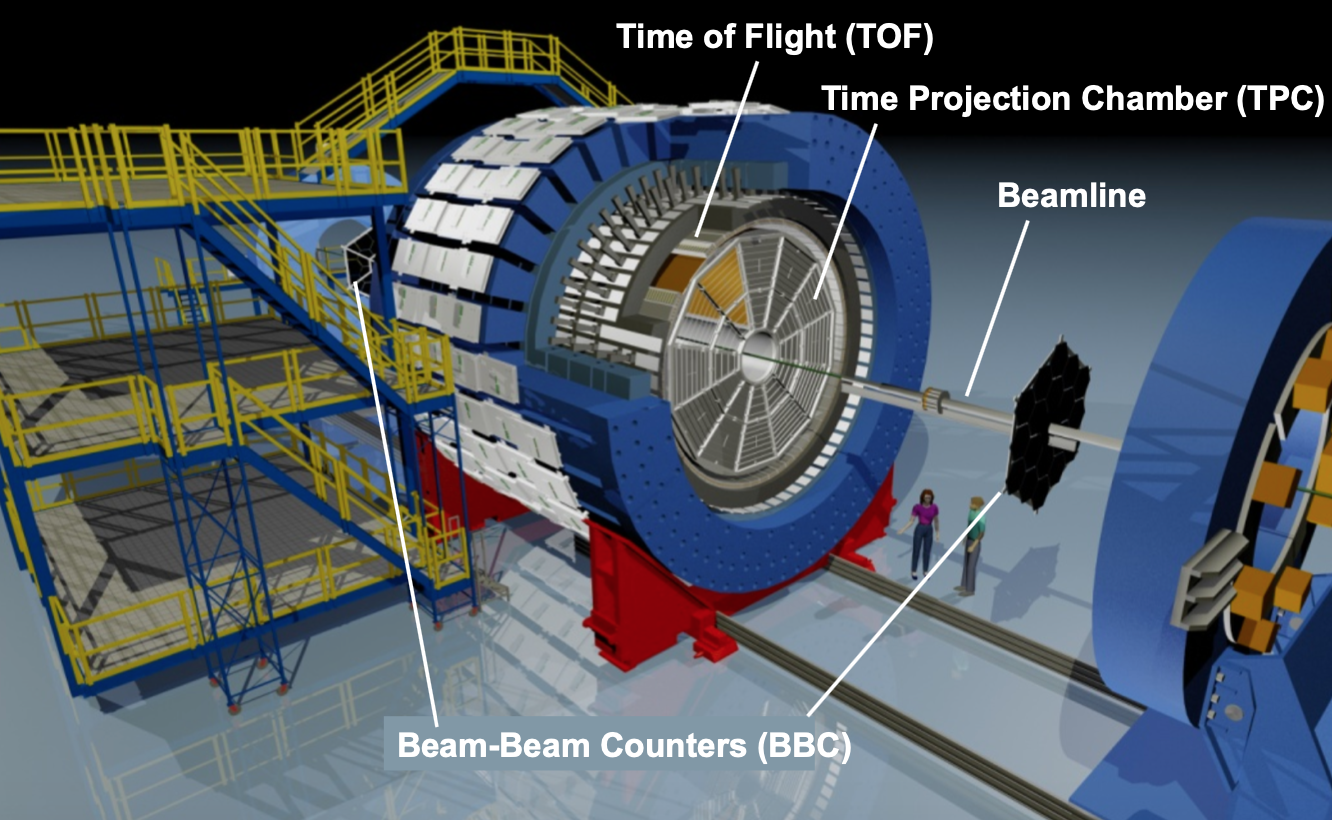
\includegraphics[width=0.4\textwidth]{Plots/STAR.png}
    \caption{\label{fig:STAR}STAR的示意图}
\end{figure}
STAR(Solenoidal Tracker At RHIC)\cite{Adams:2005dq}\cite{Adams:2003kv}作为RHIC对撞机上的一个主要探测器,如图\ref{fig:STAR}所示,由许多的次级探测器所组成,覆盖了整个方位角。在实验早期,组成STAR谱仪的探测器包括:时间投影室(Time Projection Chamber, TPC),前向的时间投影室(pair of radial-drift Forward TPC, FTPC),桶部的电磁量能器(Barrel ElectroMagnetic Calorimeter, BEMC),端部的 电磁量能器(Endcap ElectroMagnetic Calorimeter, EEMC),中央环形触发探测器(Central Scintillator Barrel, CTB),束流探测器(Beam Beam Counters, BBC),零度量能器(Zero Degree Calorimeters, ZDC),赝顶点探测器(pseudo-Vertex Position Detectors, pVPDs),环像的契伦科夫探测器(Ring-Imaging Cerenkov Retector, RICH),硅顶点探测器(Silicon Vertex Tracker, SVT)等,近年来,又增加了例如飞行时间谱仪(Time-Of-Flight detector, ToF),事件平面探测器(Event Plane Detector, EPD)和前向硅微条径迹探测器(Forward Silicon Tracker, FST)等。如图\ref{fig:STARXsec}展示了在2001年\footnote{STAR刚刚运行(2000)不久的时候。}的STAR剖面图。
\begin{figure}[htbp]
    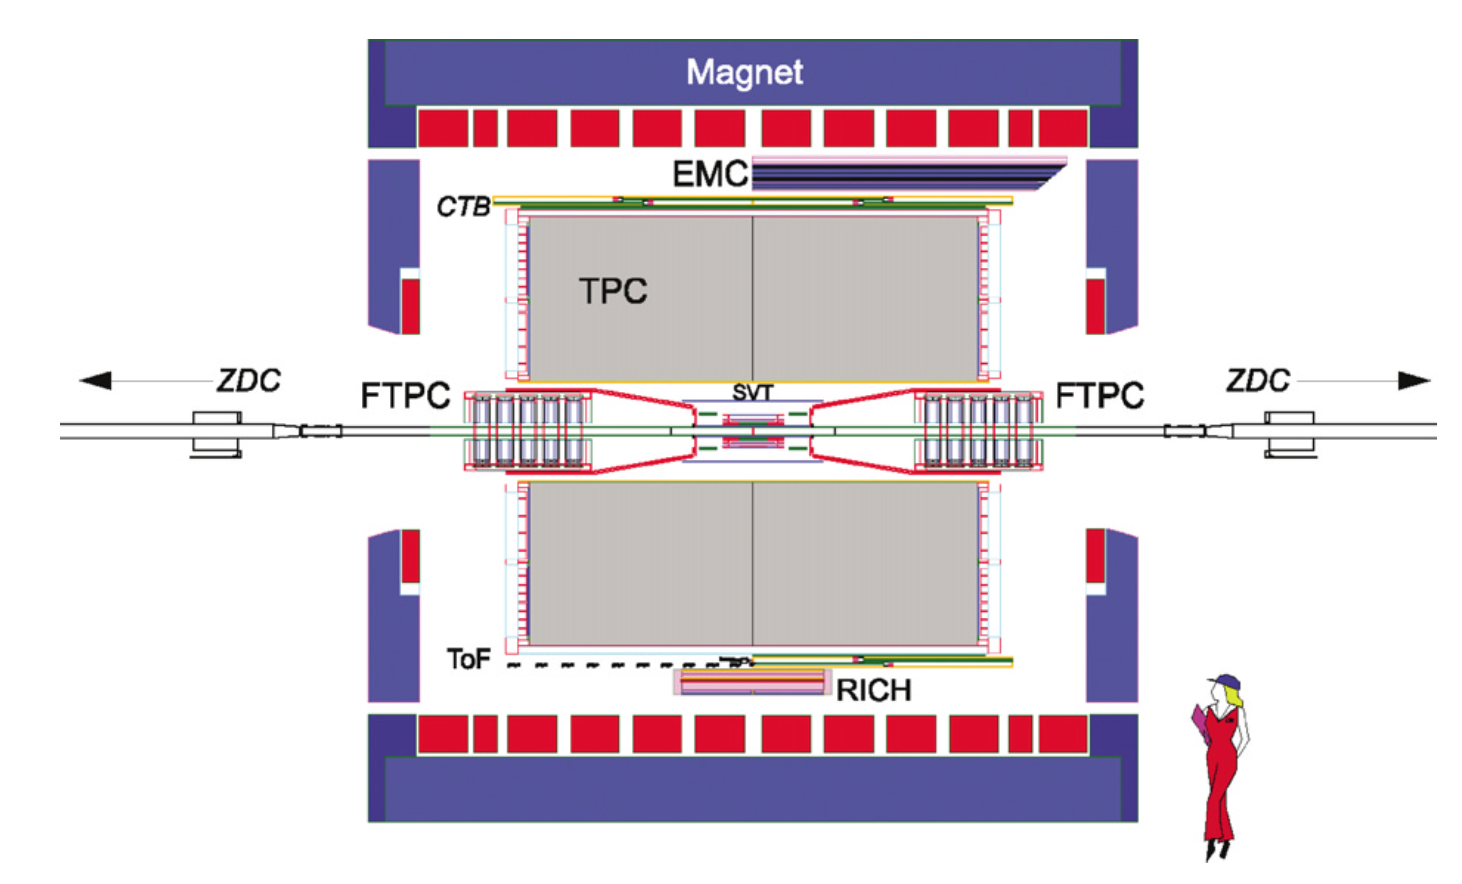
\includegraphics[width = 0.4\textwidth]{Plots/STARXsec.png}
    \caption{\label{fig:STARXsec}2001年STAR的剖面图}
\end{figure}
如图\ref{fig:STARXsec}所示,STAR的各次级探测器,基本上都集中在其环形磁铁中,STAR的环形磁铁可以提供在束流方向上的0.25到0.50T的均匀磁场。
\subsection{\label{sec:TPC}主要探测器:时间投影室}
无论是从3D模型图还是STAR的剖面图中,都可以看出,时间投影室(TPC)是STAR各个次级探测器中体积最大的,事实上,TPC也的确是STAR最为重要的次级探测器\cite{Ruan:2005hy}\cite{Dong:2005iq},这里有一个单独拿出来的示意图\ref{fig:TPC}。
\begin{figure}[htbp]
    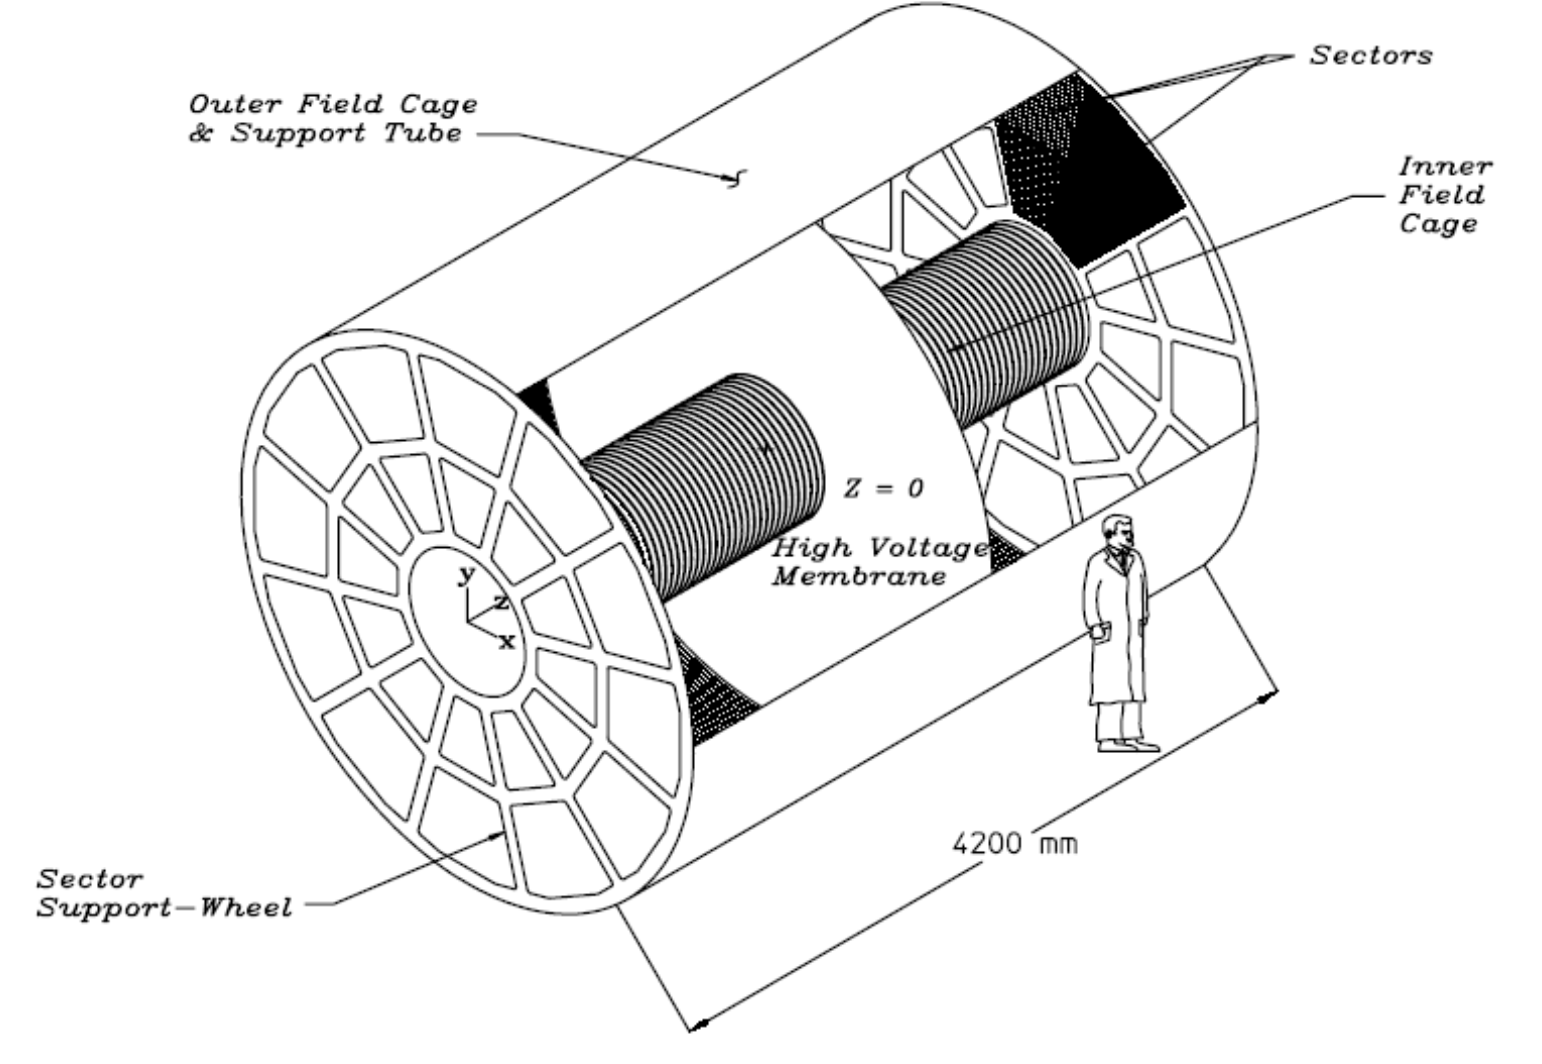
\includegraphics[width = 0.4\textwidth]{Plots/TPC.png}
    \caption{\label{fig:TPC}TPC的示意图}
\end{figure}

TPC的庞大体积,带来了令人艳羡的巨大探测范围:赝快度范围为$|\eta|<1.8$,而方位角则几乎全被覆盖,$\Delta\varphi \approx 2\pi$,从而能够测量并记录大量的碰撞产生的离子信息。从示意图中可以看出,时间投影室的几何形状是一个同心的圆环柱结构,内外径分别为$0.5\si{m}$和$2\si{m}$。在纵向上,它被分为东西两个长度均为$2.1\si{m}$漂移区,两个漂移区的体积大约为24.75m3,里面充满了混合比率为90\%的氩气和10\%的甲烷所组成的$P_{10}$气体,整个气体的压强调节在约比大气压高2mbar的范围内。在中心$Z=0$处被一个阴极膜(cathode central membrane, CM)所隔开,在中心阴极膜所加的高达$28\si{kV}$的高压,能够让被出射粒子电离出的电子与离子等在漂移区中匀速运动。在漂移区的两端则是接地的阳极读出系统,在方位角上被均分为12个区。值得一提的是,如图中接收读出区的支架,减少了约10\%的方位角覆盖。TPC探测到的径迹重建后如图\ref{fig:Eye}\ref{fig:event}。
\begin{figure}[htbp]
    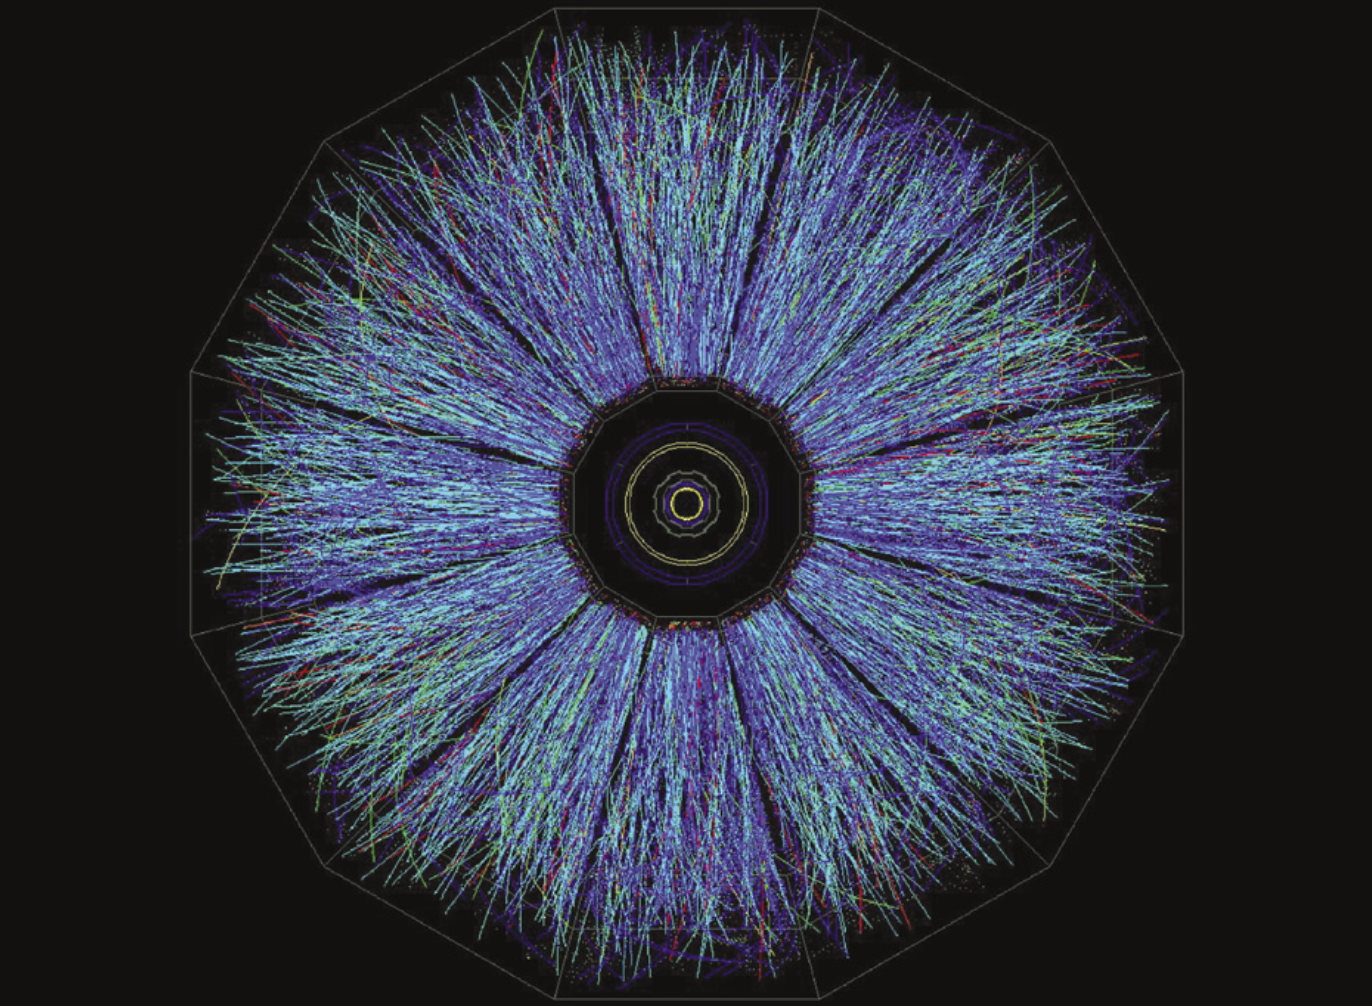
\includegraphics[width=0.4\textwidth]{Plots/Eye.png}
    \caption{\label{fig:Eye}TPC重建径迹的剖面图}
\end{figure}
\begin{figure}[htbp]
    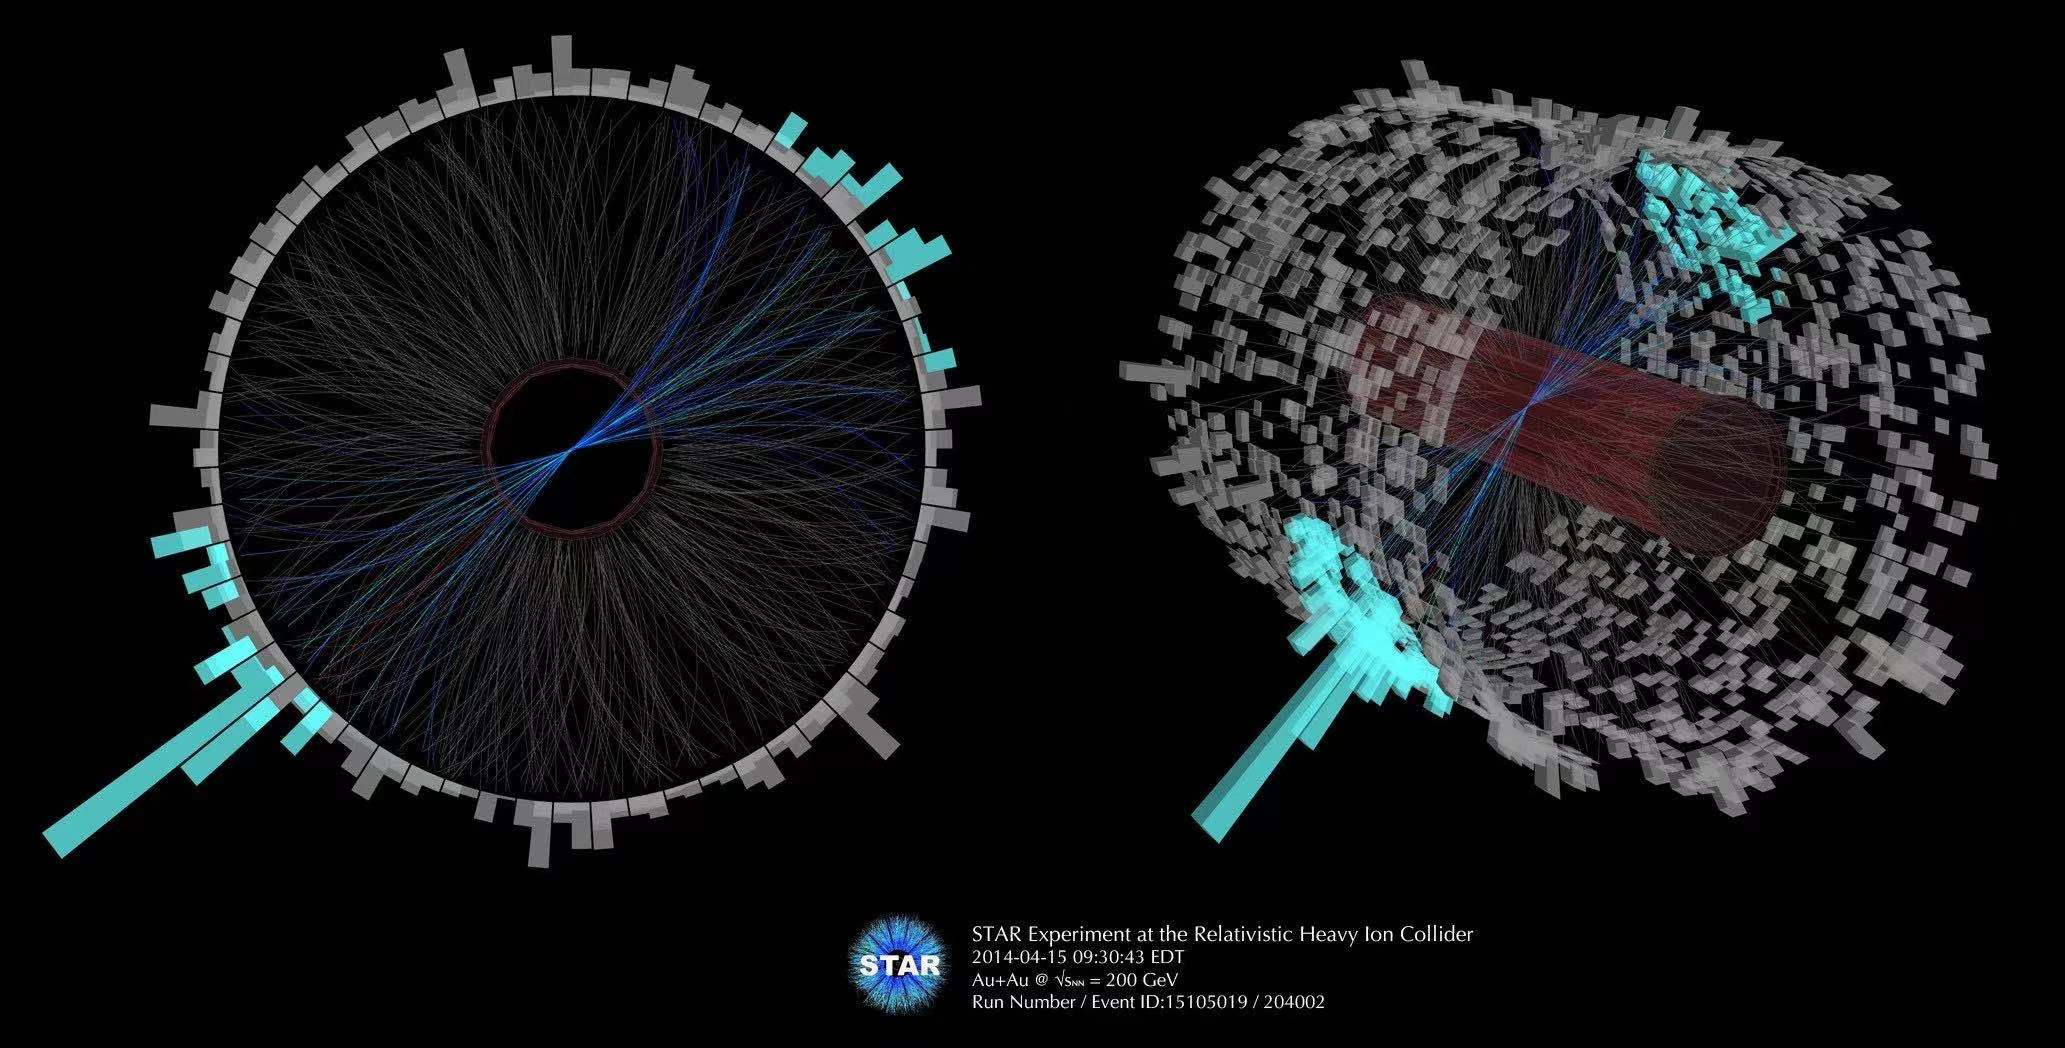
\includegraphics[width=0.4\textwidth]{Plots/event.jpg}
    \caption{\label{fig:event}TPC重建的一个事件}
\end{figure}

关于漂移室中的电离,对于高能质子对撞与重离子对撞实验中,末态带电粒子的动量主要分布在$100\si{\MeV/c}$之上。当这些带电粒子穿过TPC时,在漂移室中,这些粒子会电离出大量的电子和离子。在一个大气压左右的气压下,带电粒子在$P_{10}$气体中的能量损失本领大概是$\sim10\si{eV/cm}$数量级,从而在从TPC出射的总能量损失大概有几个$\si{MeV}$。而被这些带电粒子电离产生的电子等次级粒子,在TPC的磁场与电场的作用下,以$5.45\si{cm/\micro s}$的漂移速度做螺旋线运动向阳极漂移。

如图是一个读出区的示意图\ref{fig:TPCpad},
\begin{figure}[htbp]
    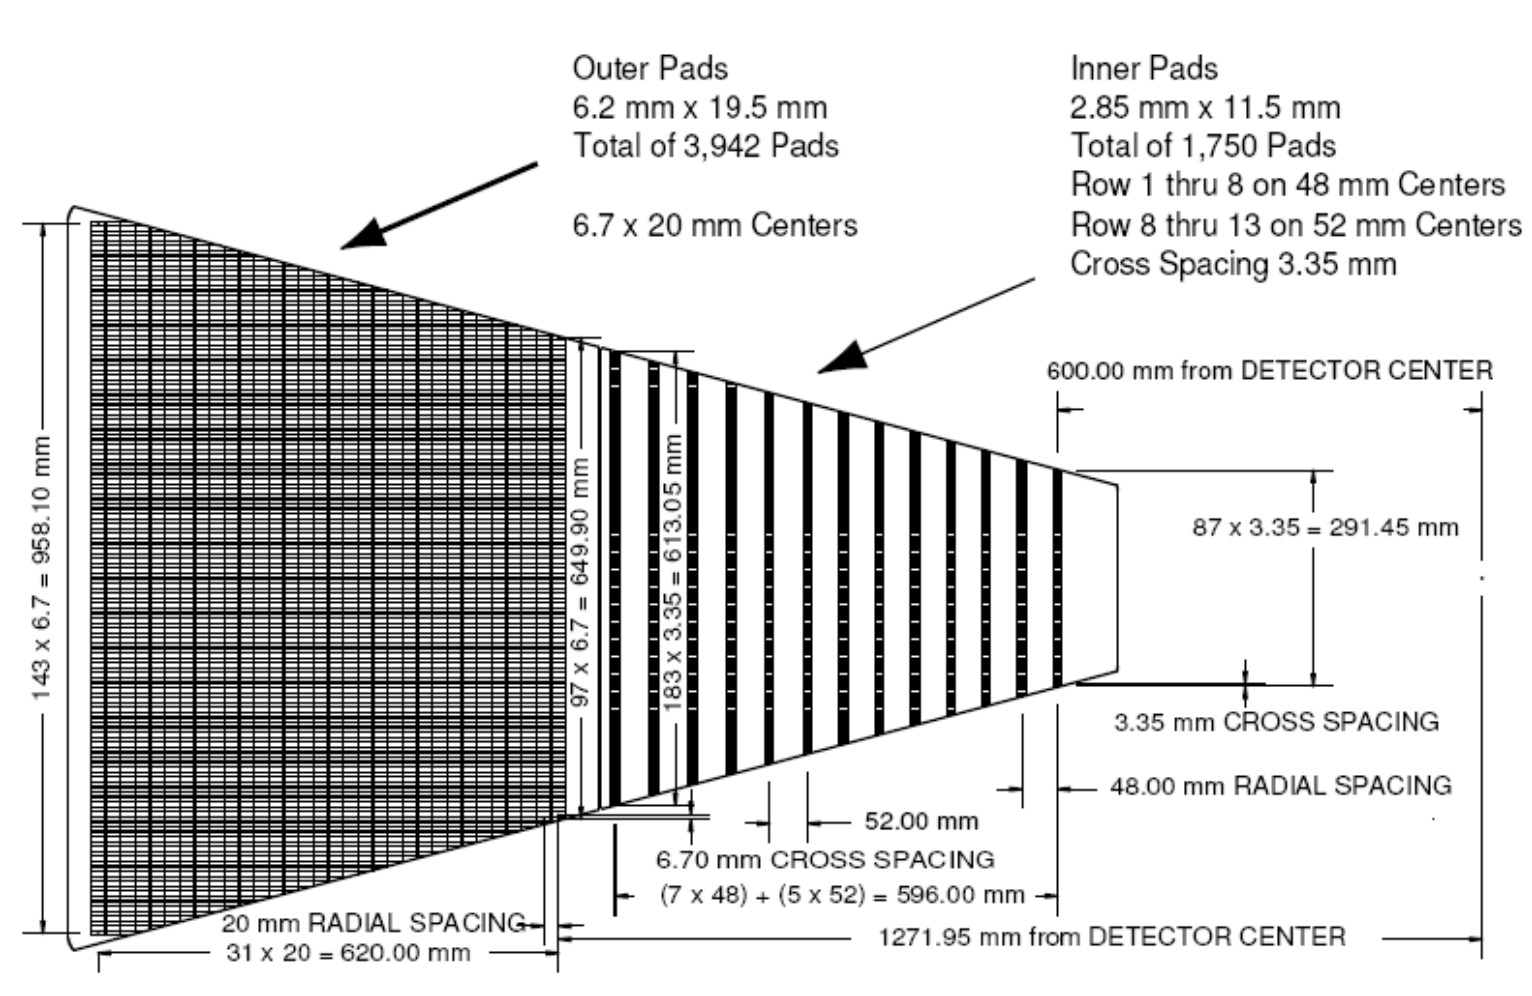
\includegraphics[width = 0.4\textwidth]{Plots/TPCpad.png}
    \caption{\label{fig:TPCpad}TPC读出区示意图}
\end{figure}
被电离出的电子等到达阳极后,信号会被放大并被接收条所接收。如图是时间投影室的接收条的分布。如前文所述,时间投影室被均分成了12份,因此一共有24个读出区。每个读出区都由小读出片组成,总计多达144,000个。每个读出区分为上下两层,上部为32排,下部则有13排,总共为45个读出排,从而能够产生最多45个信号。由于下部的带电径迹比较多,因此下部的读出片的单片面积$2.85\si{mm}\times11.5\si{mm}$比上部的读出片的单片面积$6.2\si{mm}\times19.5\si{mm}$小。这样的设计可以保证即使当粒子的多重数很大时也能给出很好的粒子径迹分辨率。

在读出区前分布有两层丝,一层有高压而另一层接地,产生巨大场强起到雪崩放大的效果。读出区下部因为信号比较强可以直接感应产生,读出区的上部则需要利用多丝正比室(MWPC)来进行读数\footnote{课程第四章内容}。通过接收的信号,人们可以得到粒子的漂移时间等,再根据漂移速度,能够重建出电离的顶点,最终获得带电粒子在TPC中的径迹(Track)。

得到径迹后,我们可以计算出径迹的曲率半径,从而计算出粒子的动力学信息等。同时,根据能量损失的Bethe-Bloch公式,不同的粒子的能量损失本领不同,对$dE/dx$进行测量,就可以对一些粒子进行鉴别,例如$\pi,K$介子之间的鉴别,和他们与质子的鉴别。除了能量损失本领的方法外,我们还可以通过弱衰变的几何分布信息,对弱衰变粒子例如$K_S^0,\lambda$介子等进行顶点的鉴别重建,又或者是通过混合事件(Event Mixing)的方法进行强衰变粒子如$K^*,\phi,\Delta$的鉴别。

当然,TPC也有其不足之处,对于低动量出射粒子的情况,因为容易衰变而使时间投影室不能探测到。而在高的横动量时,各种粒子的电离损失的能量又基本一致,结果是时间投影室的横动量分辨范围对于$\pi,K$介子只能达到 $600\si{MeV\per c}\sim700\si{MeV\per c}$。而对于质子和反质子只能达到$1.0\si{GeV\per c}\sim1.1\si{GeV\per c}$\ref{fig:dEdx}。
\begin{figure}[htbp]
    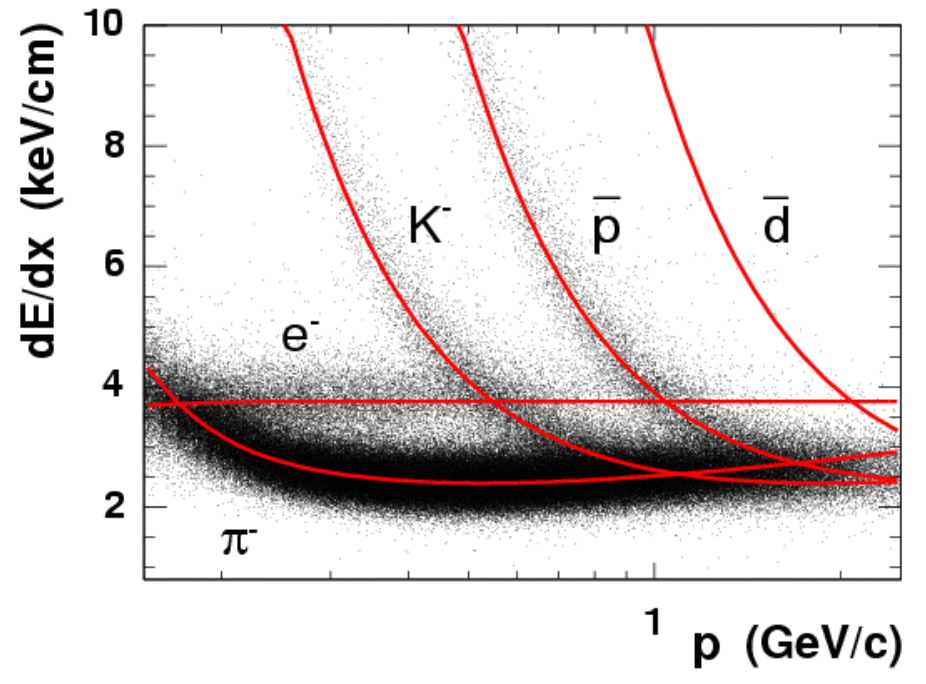
\includegraphics[width=0.4\textwidth]{Plots/dEdx.png}
    \caption{\label{fig:dEdx}TPC的能损分辨本领}
\end{figure}
\subsection{\label{sec:ToF}重要探测器:飞行时间谱仪}
如前文所述,TPC作为STAR的主要探测器有着许多优越的性能,但是,STAR也需要次级探测器来提高TPC的鉴别精度。这些为接下来要叙述的飞行时间谱仪(ToF)提供了背景。

STAR的ToF主要由中国科学技术大学负责设计\cite{Cheng}\cite{Ruan:2005hy}。传统来说,ToF一般由塑料闪烁体与光电倍增管组成。但是,由于STAR的覆盖面积太大,满足需求的传统ToF造价太高。鉴于在相对论性重离子碰撞中,大家大多关心末态粒子中的带电粒子,STAR提出用多层电阻板室(Multi-gap Resistive Plate Chamber,MRPC)来建造飞行时间探测器。

用来建造飞行时间谱仪探测器的多层电阻板室具有六个220$\si{\micro m}$的间隙,它同时拥有六个读出条,每个读出条的面积约为$60\times32\si{mm\square}$。 多层电阻板室的示意图如图\ref{fig:MRPC}。
\begin{figure}[htbp]
    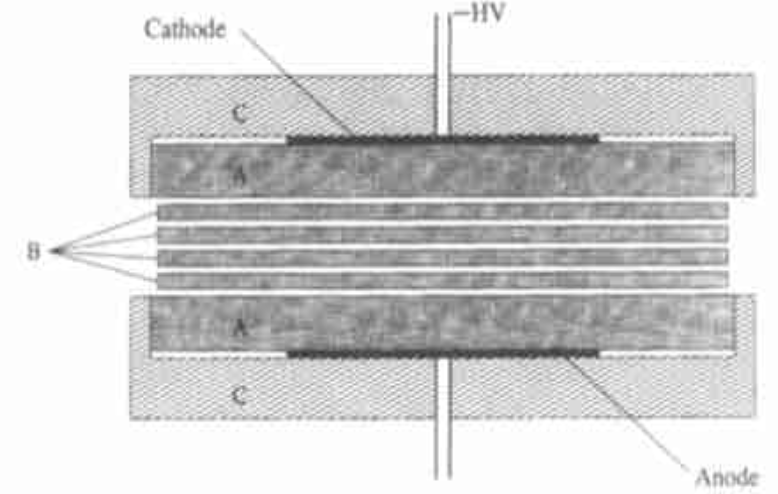
\includegraphics[width=0.4\textwidth]{Plots/MRPC.png}
    \caption{\label{fig:MRPC}多层电阻板室示意图}
\end{figure}
其主要由高压电极,电阻板层,气隙,读出层和Mylar膜和框架组成。在固定的框架内,最外面的为两个读出层,读出层由上下两个印刷线路板构成,它们上面分别镀上金的感应电极。高压层在读出层的里面,它为一层石墨胶带,上面加上了几千伏的高压。为了防止高压层和读出层之间短路,读出层和高压电极之间加上了一层绝缘的Mylar膜。 在高压层的里面为五块电阻板层,它们由$0.7\si{mm}$厚的玻璃构成,它们中间夹着细的鱼丝,来维持恒定的间距。整个室被五块电阻板层分为六个$220\si{\micro m}$的气隙。气隙中充入$\text{SF}_6$,$\text{C}_4\text{H}_{10}$和$\text{F}_{134}\text{A}$的混合气体。它们的体积比例为1:1:18。

相比于利用传统的利用光电倍增管的ToF,工作原理上MRPC反而和传统的气体探测器有些类似。利用高压层上的高压形成一个平行电场,五块电阻板层不与高压层连接而是悬浮在电场中。当粒子穿过室时,在中间的气隙中会发生电离,产生原初电离粒子。由于我们所加的高压很高,因此在气隙中间的电场的作用下,原初电离粒子在很短的距离就可以发生雪崩电离,从而达到电子倍增的效果。事实上。整个MRPC的主要工作区基本为正比雪崩放电区。各个间隙内雪崩放电产生的电子沿电场漂移,最终被电阻板层所阻断。由于充入的为混合的重气体,因此在探测器中,原初电离约为100cluster/mm。原初电离符合泊松分布,因此我们可以测算在贴近电阻板层的几十微米的区域发生原初电离的几率是接近98\%。因此 MRPC的探测效率接近百分之百。由于电阻板层是由玻璃构成,它在高压下有半导体的属性电阻值很高,体电阻一般在$10^{11}\sim10^{12}$欧姆,并且电阻板在电场中处于悬浮电位,这样就能保证对电磁场的传播是基本透明的。因此雪崩电离的粒子可以靠电磁感应把信号局域地传递给相应的读出信号,速度非常快。这样影响MRPC时间分辨的因素主要为最初几个原初电离粒子在气隙中位置的晃动。由于MRPC的气隙只有几百 微米,因此电子的漂移距离非常小,造成的时间的晃动很小。因此MRPC的时间分辨也非常的高。

基于MRPC的ToF有着如此之高的时间分辨能力,它可以将整个 STAR 的粒子鉴别能力提高到一个很高的范围。根据测量得到的 MRPC 的时间分辨$\sigma=80\si{ps}$, 对 MRPC-ToF 的粒子鉴别能力的模拟结果显示如图\ref{fig:ToF},
\begin{figure}[htbp]
    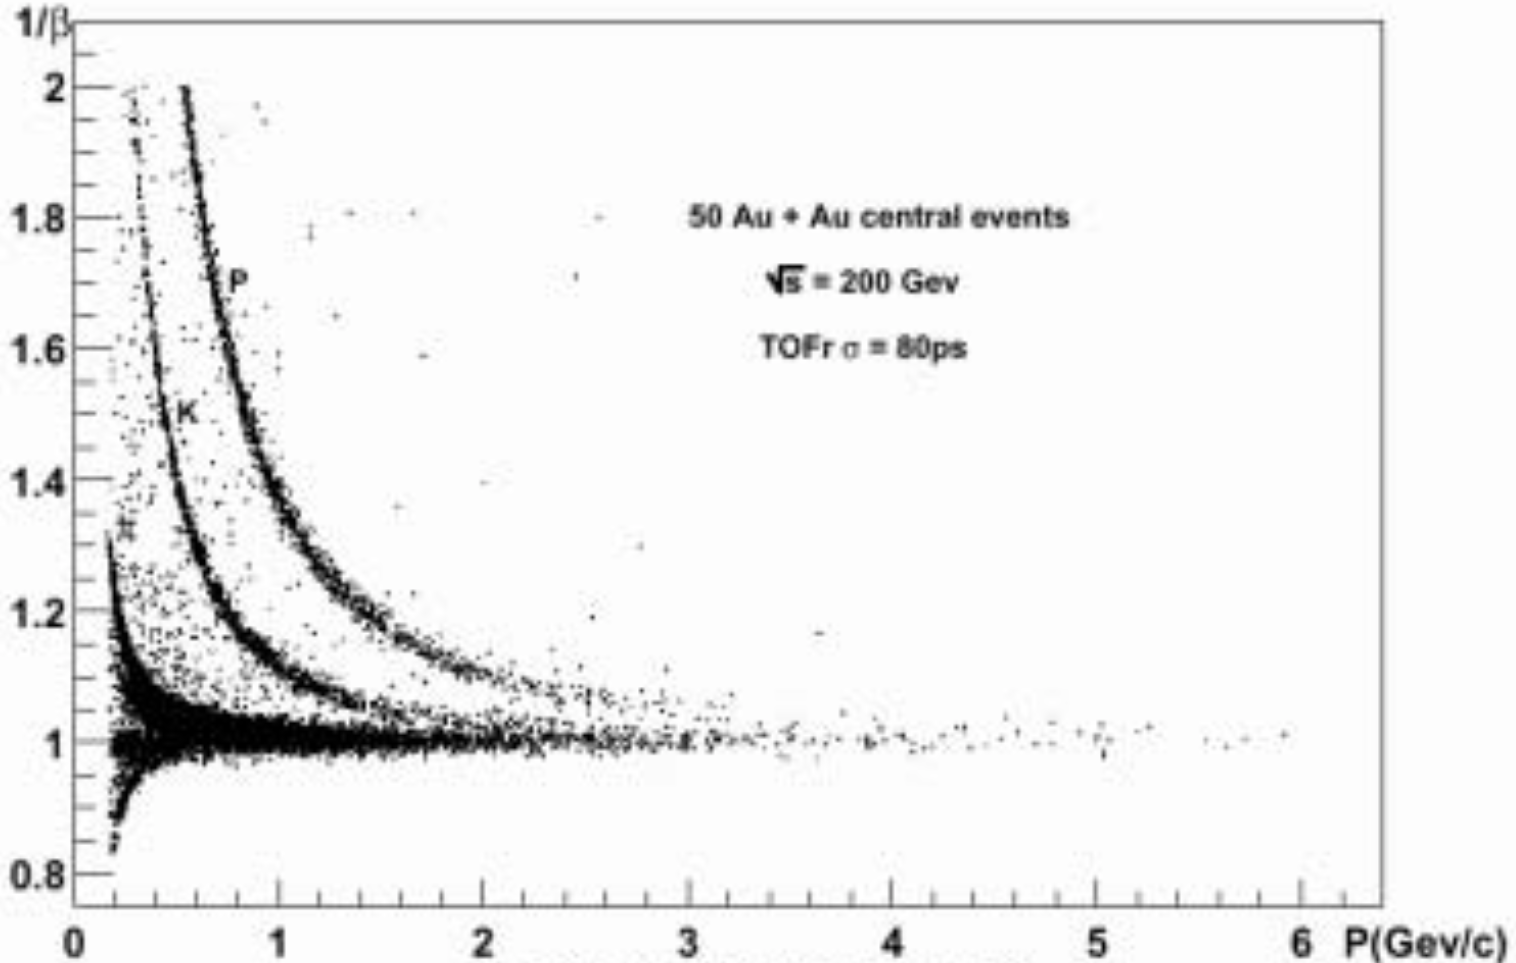
\includegraphics[width = 0.4\textwidth]{Plots/dEdxToF.png}
    \caption{\label{fig:ToF}ToF的能量损失分辨本领}
\end{figure}
图中内容为$200\si{GeV}$的Au-Au中心对撞中,速度的倒数和动量的关系。从这张图中可以看出,MRPC-TOF 是一个比较清晰的探测器,能够很清楚的看到$\pi,K$介子以及质子和反质子。并且在很高的动量下,粒子的鉴别依然很好。进一步的模拟显示,MRPC-ToF 对于$\pi,K$介子的鉴别能力可以达到$1.7\si{GeV/c}$以上.对于$K$介子和质子(反质子),鉴别能力可以达到$2.4\si{GeV/c}$以上,这将鉴别几乎所有Au-Au碰撞产生的质子。

\section{\label{sec:PhyRes}STAR的物理结果}
\subsection{\label{sec:qgp}QGP的物理性质}
STAR探测器是为了探测QGP的性质而设计的,而后来的实验证据表明,STAR很好的达到了设计的预期。下面我将介绍STAR与QGP相关的一些主要结果。
\subsubsection{\label{sec:Flow}集体流}
如果去翻阅STAR的出版物历史,集体流的测量可以称得上是STAR的开山之作\cite{Ackermann:2000tr}。在这里,集体流指的是相对论性重离子碰撞中末态粒子动量分布的集体性,后来又被在小碰撞系统,如非对称的小核(氢,氘,氚)与金、铅等大核碰撞,或者甚至是质子对撞系统中所观测到。

集体流测量的基本观测量是集体流系数(Flow harmonics),
\begin{equation}
    \langle \frac{d^3N}{d^3 p} \rangle = \frac{1}{2\pi} \langle \frac{d^2N}{p_Tdp_Td\eta} (1+\sum_{n=1}^\infty v_n(p_T,\eta)\cos(n(\varphi-\psi_r))) \rangle 
\end{equation}
可以看作是对末态粒子分布对方位角$\varphi$进行傅立叶分解,来得到横平面各阶几何信息。式中的$\psi_r$是所谓的事件反应平面角(reaction plane angle),可以视为对于特定的碰撞事件,初态与实验室参考系定义的x-y的偏转角。

除了上式展示的微分流形式,我们还可以对横动量$p_T$和赝快度$\eta$积分,得到积分流
\begin{equation}
    \langle \frac{dN}{d\varphi} \rangle = \frac{1}{2\pi} \langle (\sum_{n=0}^\infty V_n\cos(n(\varphi-\psi_r))) \rangle 
\end{equation}
显然的,式中的$V_0$给出了粒子的产额,一般来说,实验中会选择测量
\begin{equation}
    v_n = \frac{V_n}{V_0}
\end{equation}
这一归一化后的集体流系数来衡量体系的各向异性。

集体流的物理意义如同其定义一般明晰,如图\ref{fig:Config}\cite{Qiu:2013wca}给出了一个相对论性重离子碰撞事件的初态构型,
\begin{figure}[htbp]
    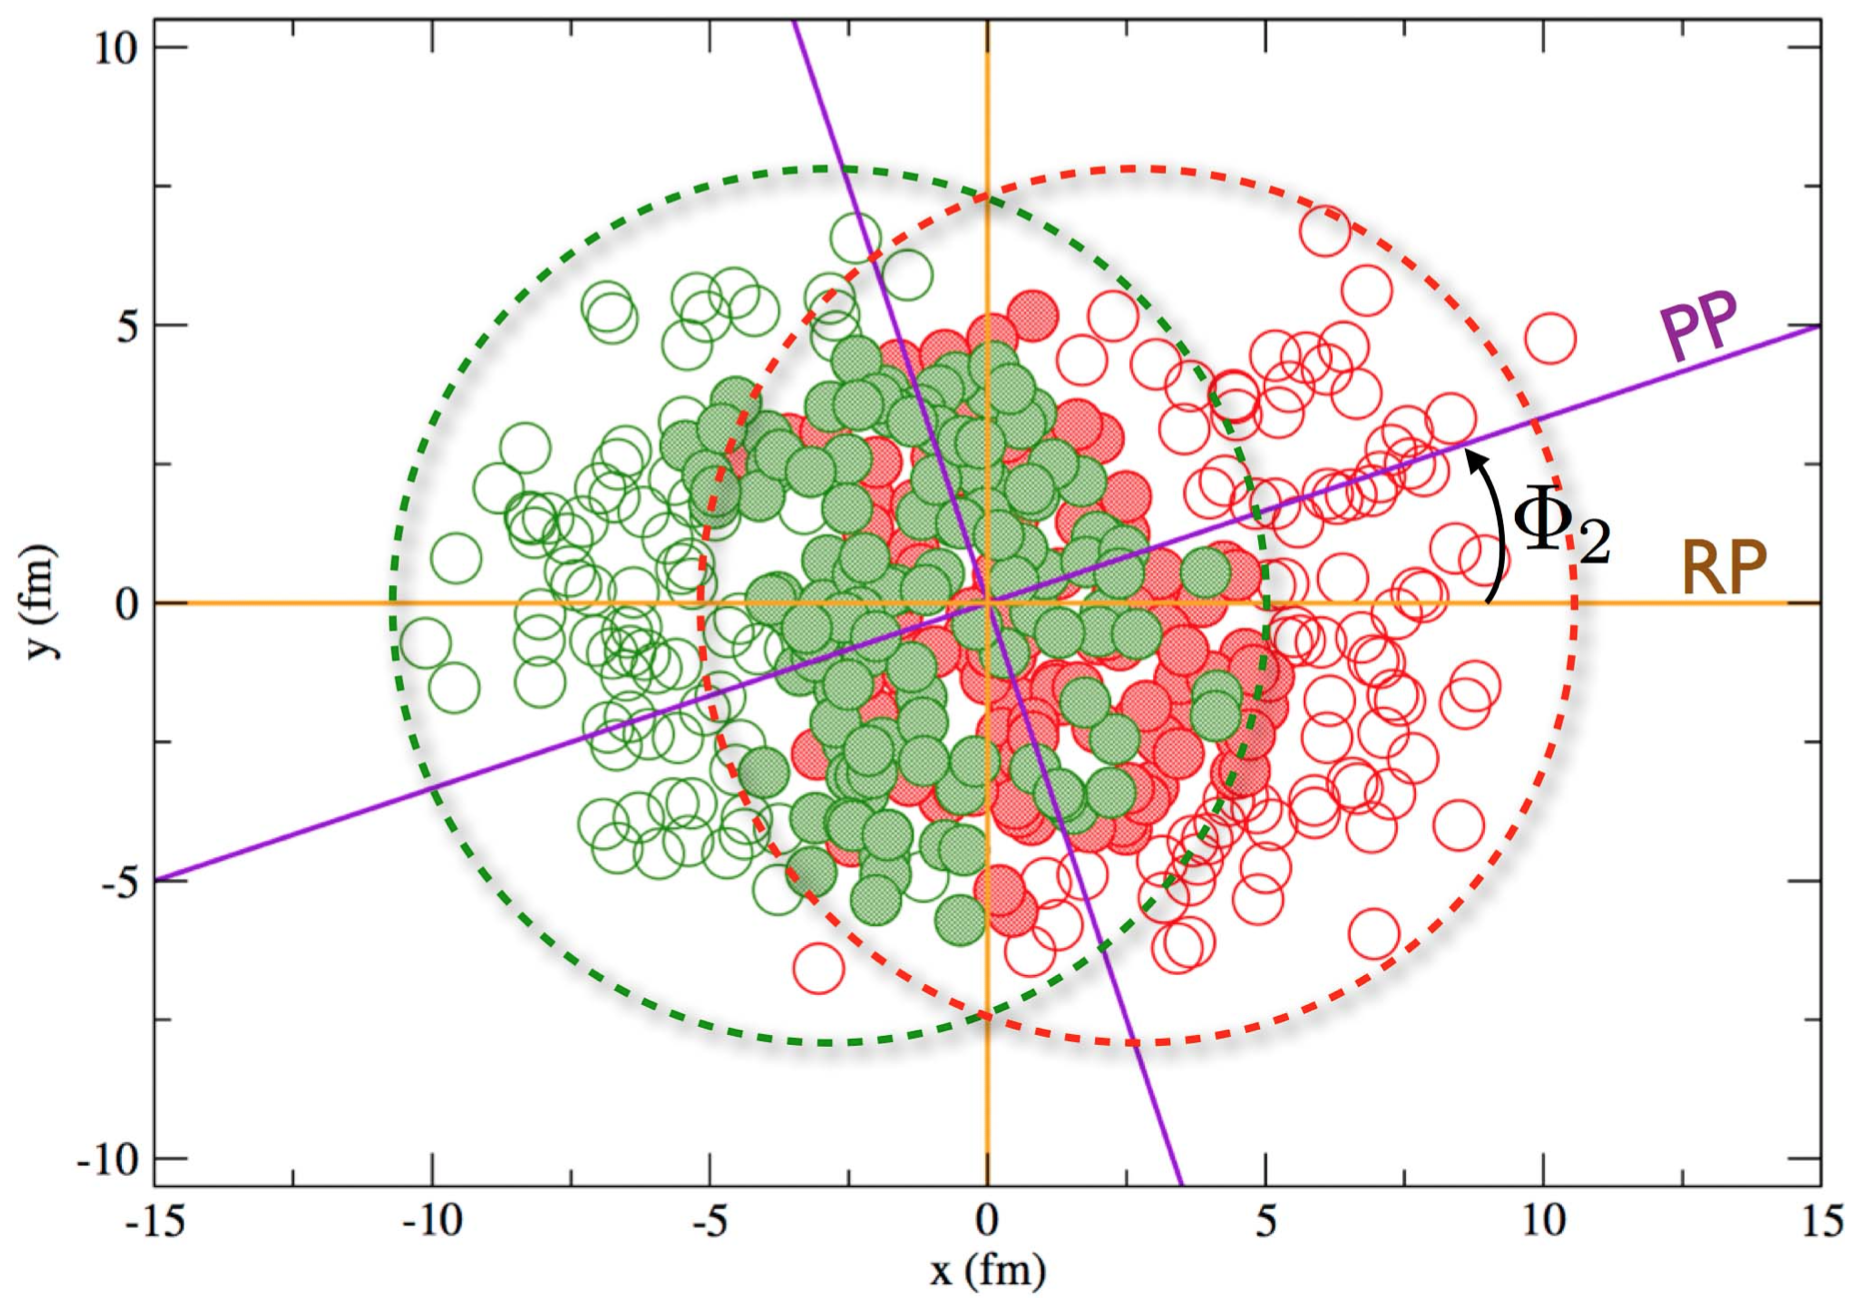
\includegraphics[width=0.4\textwidth]{Plots/Config.png}
    \caption{\label{fig:Config}一个相对论性重离子碰撞事件的初态核子构型}
\end{figure}
不难想象,根据碰撞参数(Impact Parameter)的不同,中心的重叠部分,尽管都是一个类似椭圆的形状,但其二阶离心率(Eccentricity)\footnote{这里的离心率是一个广义的概念,而不是说中心重叠部分真的是一个椭圆}$\varepsilon_2$是一个逐事件涨落的随机变量。经过QGP内部胶子和夸克之间相互作用的传导,这一坐标空间的各向异性会引发末态动量空间的各向异性如图\ref{fig:v2e2}\cite{Zhou:2020pai}。
\begin{figure}[htbp]
    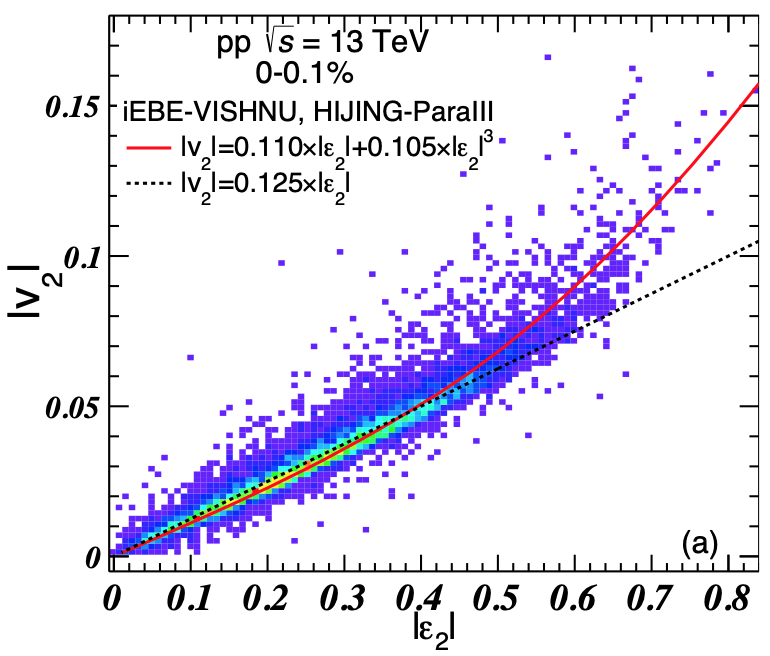
\includegraphics[width=0.4\textwidth]{Plots/v2e2.png}
    \caption{\label{fig:v2e2}相对论性重离子碰撞中初末态各向异性的响应}
\end{figure}

如图\ref{fig:v2}展示了STAR对二阶流的首次测量结果\cite{Ackermann:2000tr},
\begin{figure}[htbp]
    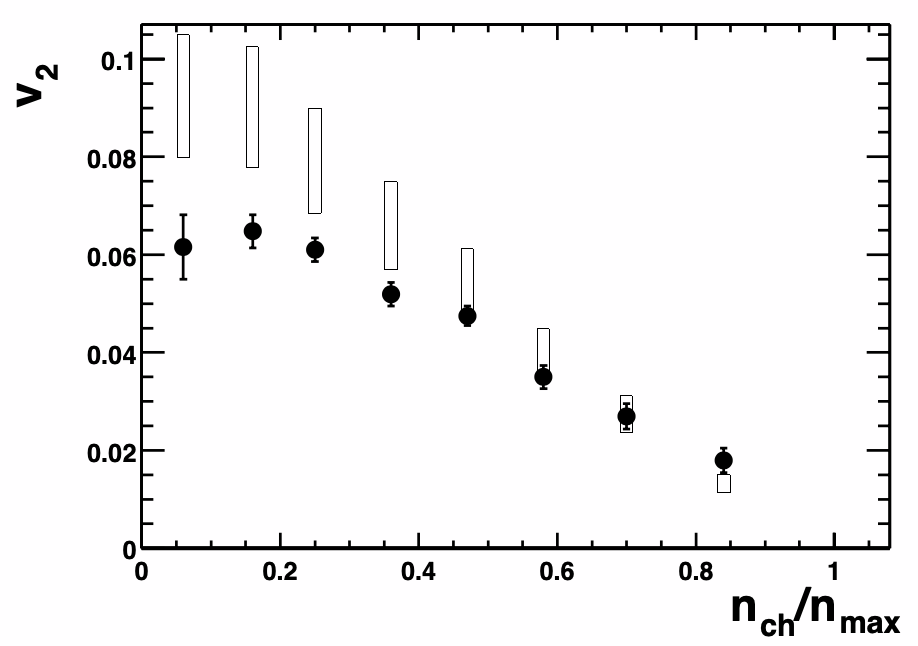
\includegraphics[width=0.4\textwidth]{Plots/v2.png}
    \caption{\label{fig:v2}STAR对集体流的首次测量:积分流}
\end{figure}
横轴是事件的总带电粒子多重数(Multiplicity of Charge Particle)$n_{ch}$除以最大值$n_{max}$,这一比值是通过末态产出定义事件的中心度(Centrality)。图中实心点是实验的测量结果,而空心的矩形则是当时的流体力学(Hydrodynamics)给出的预测。在文章的最后总结部分指出,相比于先前的较为低能的重离子固定靶实验(SPS, AGS)等,在高能情形下,相比于相对论性量子分子动力学(RQMD)的预测,基于流体力学的预测能够更好的解释实验数据,这侧面证实了高能重离子对撞下系统的热化(Thermalization)已经比较完全\footnote{至少在非边缘碰撞事件为代表的大系统中}。换句话说,系统已经达到了局域平衡态,这一现象支持了QGP物质间的相互作用。

在之后的实验中,相对论性重离子碰撞为QGP的性质提供了一个又一个有力的约束。举例来说,如图\ref{fig:v2pt}\cite{Ackermann:2000tr}所限展示的在高横动量区域的压低,
\begin{figure}[htbp]
    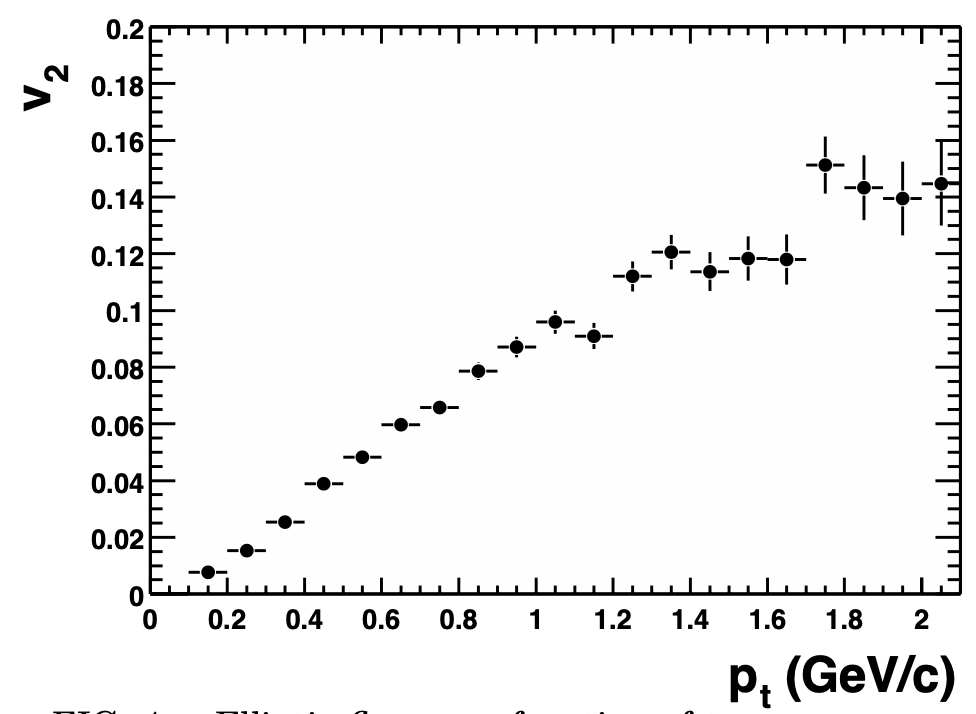
\includegraphics[width=0.4\textwidth]{Plots/v2pt.png}
    \caption{\label{fig:v2pt}STAR对集体流的首次测量:横动量微分流}
\end{figure}
其背后暗示了在QGP自身的粘滞效应(Viscosity),这一效应不仅和流体力学建模相关。在所谓的反德西特时空与共性场论对偶理论(AdS/CFT)预言下,一个强相互作用费米子系统的剪切粘滞系数$\eta/s$存在下限(式中为自然单位制)
\begin{equation}
    \eta/s \leq \frac{1}{4\pi}
\end{equation}
而在人们发展了粘滞流体力学模型后,模型预言的粘滞系数,恰好就位于这一极限附近。
\subsubsection{其他流体性质}
一般来说,在STAR的QGP性质测量都需要利用前向探测器而不仅仅是TPC和ToF,除了集体流\footnote{事实上眼下的集体流分析也需要前向探测器。},在这里不进行详细介绍。
\begin{description}
    \item[喷注淬火(Jet Quenching)] 喷注(Jet)是对撞机上的常见现象,由于QCD紧闭效应,人们并不能看到裸夸克或胶子,而是看到一簇簇强子束。由于动量守恒,我们通常能够在横平面(Transverse Plane)上看到所谓的背靠背喷注(Back-to-Back Jet)。然而,在相对论性重离子对撞实验中,一个常见的现象是一对背靠背喷注中的一支射入了QGP,在和介质相互作用出射后强度降低甚至消失。这一现象可以被所谓的核修正因子($R_{AA}$)所描述:
    \begin{equation}
        R_{AA}(p_T) = \frac{d^2 N^{AA}/dp_Td\eta}{T_{AA}d^2 \sigma^{NN}/dp_Td\eta},T_{AA} = \langle N_{bin} \rangle/\sigma^{NN}_{inel}
    \end{equation} 
    $R_{AA}$的物理意义,可以理解为实验上所观测到的强子谱,与把重核碰撞当成核子间碰撞得到的强子谱组合间的比值。

    如图\ref{fig:RAA}展示了STAR的测量结果\cite{Adams:2003kv},
    \begin{figure}[htbp]
        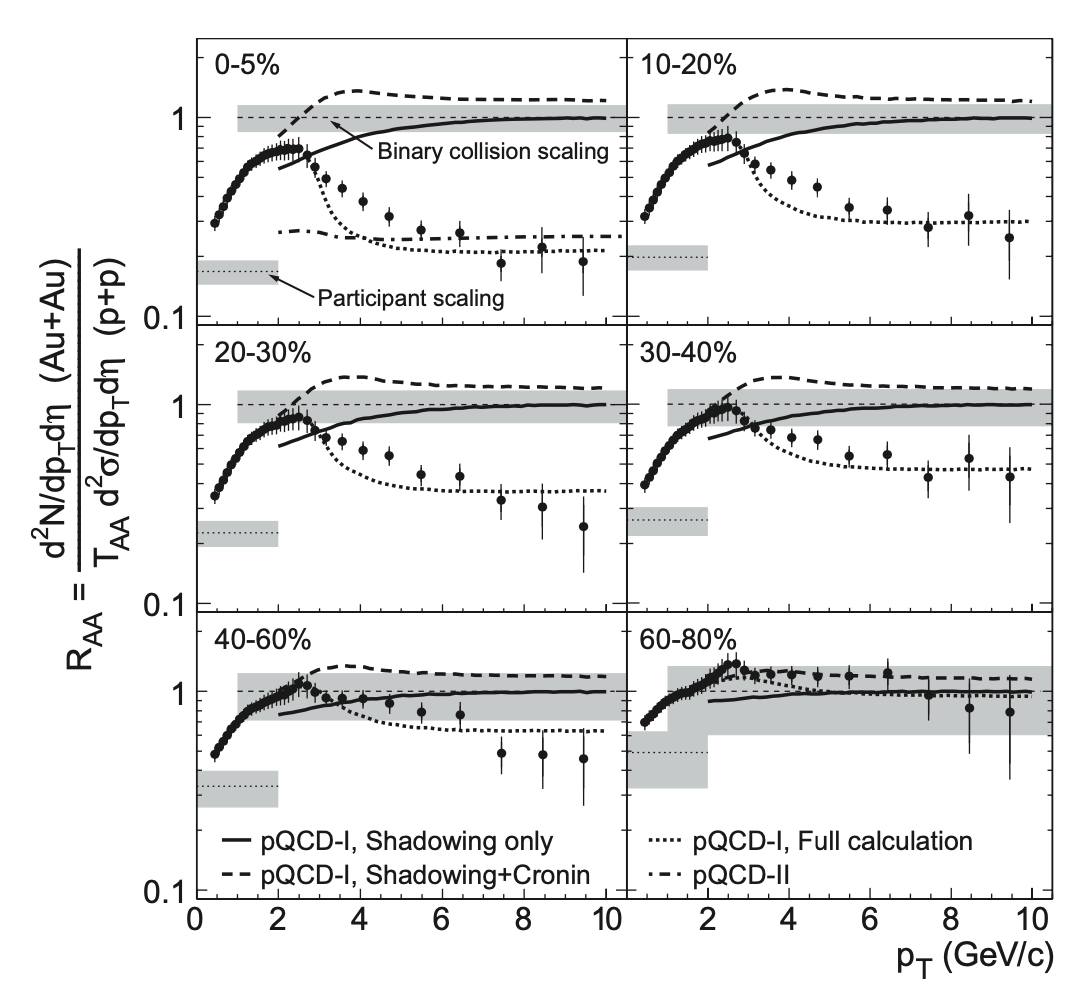
\includegraphics[width=0.4\textwidth]{Plots/RAA.png}
        \caption{\label{fig:RAA}核修正因子的测量结果}
    \end{figure}
    可以看出,在高横动量区间有着明显的压低效应,同时注意到,核修正因子的预测在微扰QCD下计算还是有一些不足之处。
    \item[$\Lambda$ 极化($\Lambda$ Polarization)] 涡旋$Vortex$是流体力学研究的一个重要方面,代表了角动量效应。既然QGP的性质接近于液体,同时在相对论情形下有着极大的角动量,人们就开始期待是否能够对QGP中的涡旋效应进行测量。在这里,一个简单的方法是,考虑到轨道角动量和自旋的耦合,通过测量末态的极化,就能够探测到背景流体的涡旋结构。
    
    通过测量$\Lambda$超子的极化\cite{STAR:2017ckg}如图\ref{fig:Lambda},
    \begin{figure}[htbp]
        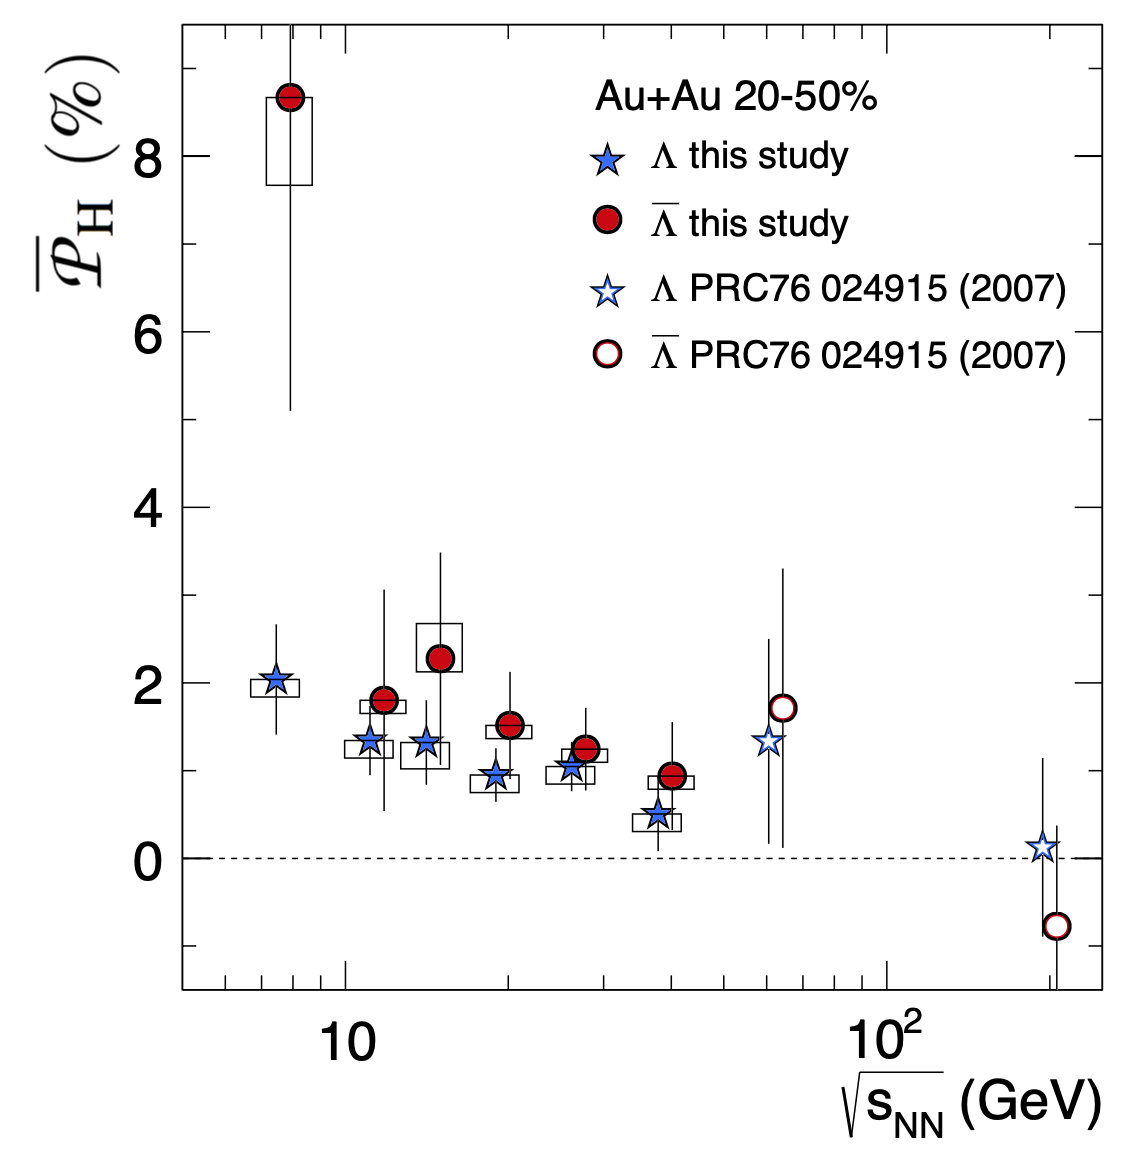
\includegraphics[width=0.4\textwidth]{Plots/Lambda.png}
        \caption{\label{fig:Lambda}$\Lambda$极化的测量结果}
    \end{figure} 
    STAR观测到了显著非零的极化效应,从而有力的证明了QGP中存在涡旋。
\end{description}
\subsection{\label{sec:antimatter}反物质产生}
通过TPC和ToF,STAR能够做到良好的粒子鉴别效果。这不仅让人们能够测量到QGP背景下的各种强子产生,还能够探测相对论性重离子碰撞的高能环境下产生的反粒子。
\subsubsection{\label{sec:antihypertritons}反超氢}
对于(反)超氢$^3_\Lambda \text{H}(^3_{\bar\Lambda} \overline{\text{H}})$,一般利用这一衰变过程
\begin{equation}
    ^3_\Lambda \text{H}(^3_{\bar\Lambda} \overline{\text{H}}) \to  ^3\text{He}(^3\text{He})+\pi^-(\pi^+)
\end{equation}
进行探测。

在分析\cite{Abelev:2010rv}中,利用TPC重建的鉴别了粒子的径迹数据,人们可以重建出$^3\text{He}(^3\text{He})$和$\pi^-(\pi^+)$的径迹,再通过衰变顶点的几何进行筛选,最后重建出$^3\text{He}-\pi^-(^3\text{He}-\pi^+)$的不变质量如图\ref{fig:Hyperon}。这一不变质量峰也就显示出(反)超氢的产生。
\begin{figure}[htbp]
    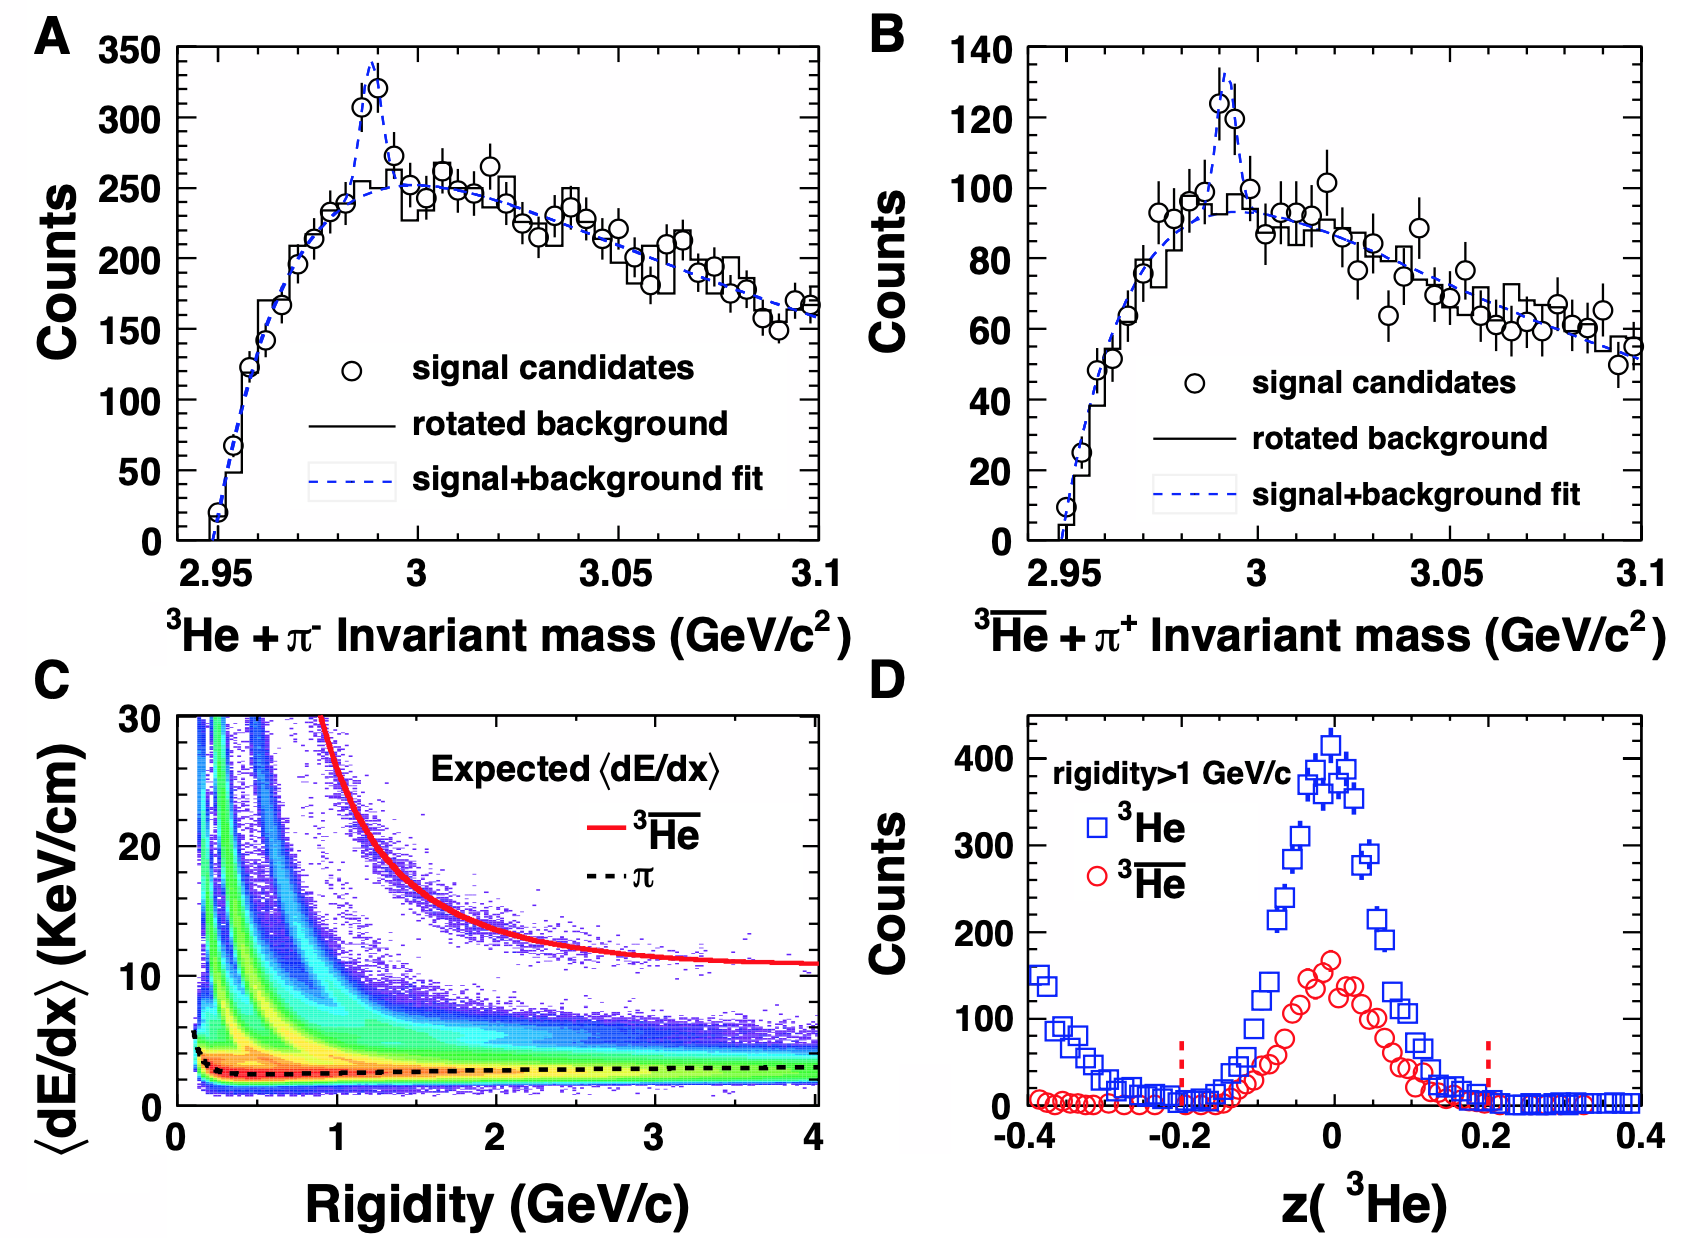
\includegraphics[width=0.4\textwidth]{Plots/Hyperon.png}
    \caption{\label{fig:Hyperon}反超氢的测量}
\end{figure}
\subsubsection{\label{sec:antihelium4}反氦四}
相比于反超氢,反氦四的观测\cite{Agakishiev:2011ib}更加直接,可以直接通过如图\ref{fig:dEdxAll}\ref{fig:dEdxHe4}的能损本领进行粒子鉴别。
\begin{figure}[htbp]
    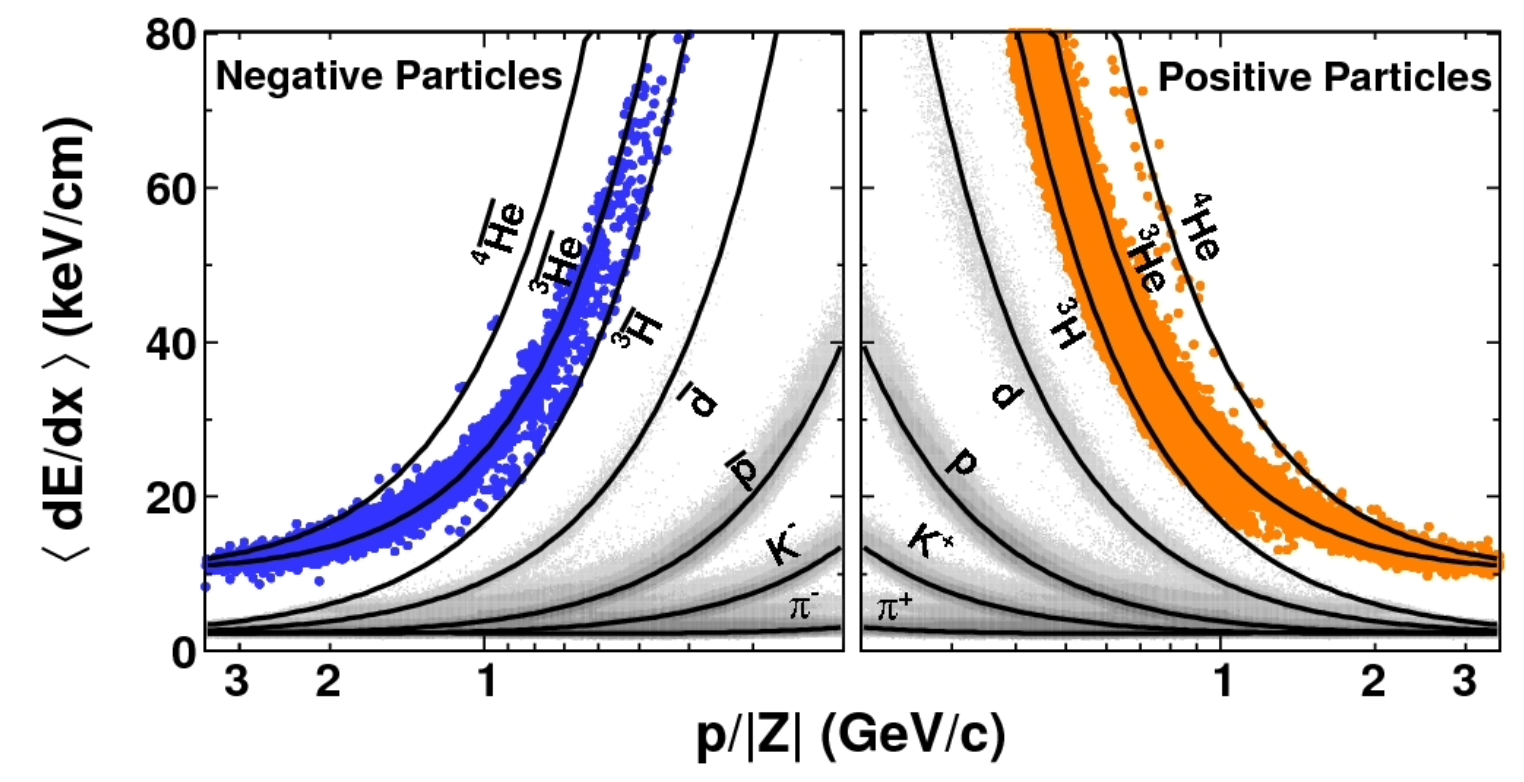
\includegraphics[width=0.4\textwidth]{Plots/dEdxAll.png}
    \caption{\label{fig:dEdxAll}整体的能损分辨本领}
\end{figure}
\begin{figure}[htbp]
    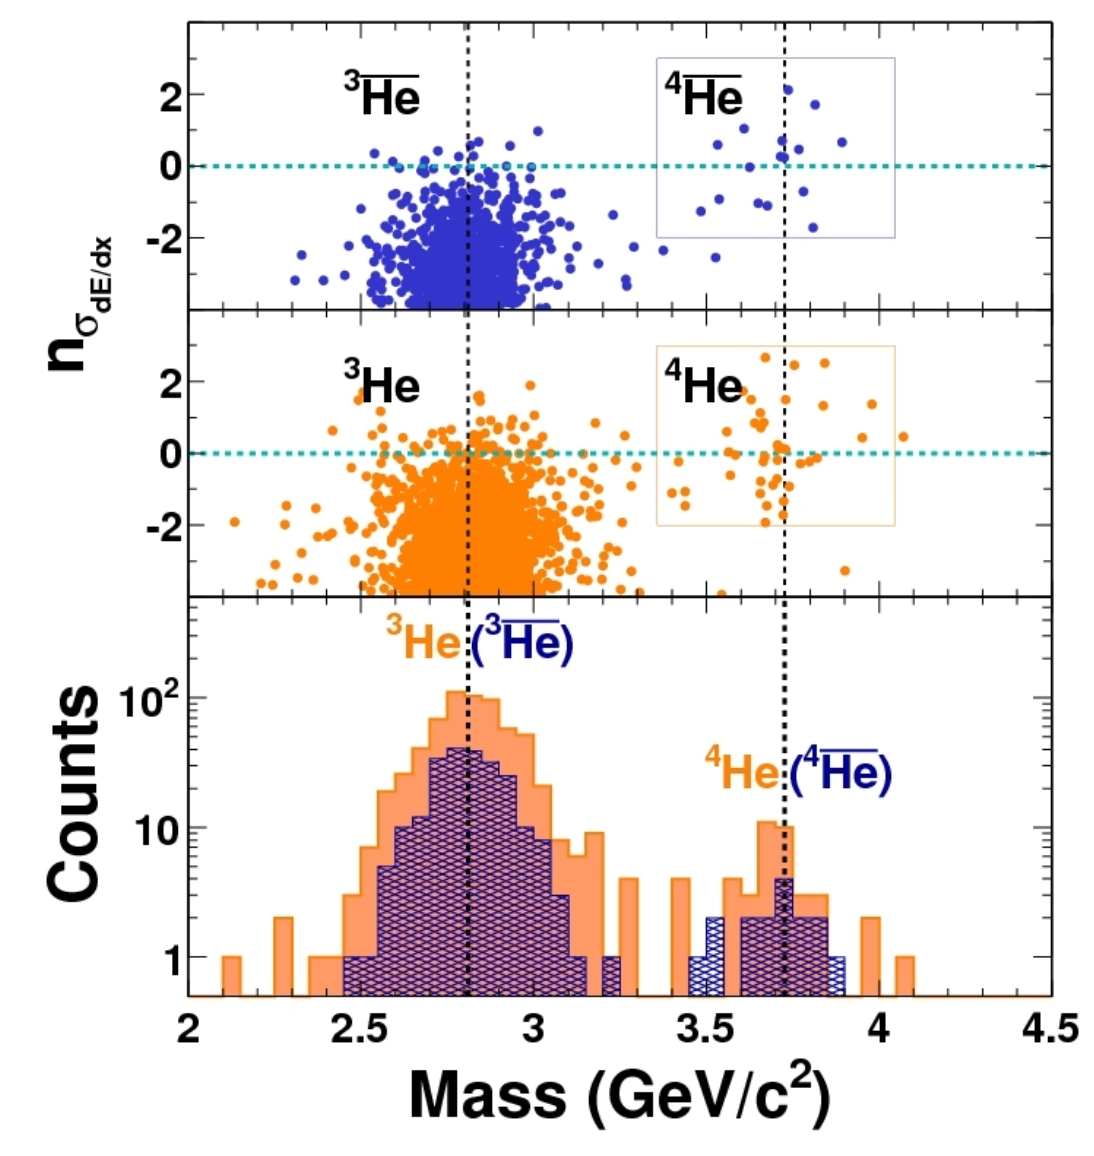
\includegraphics[width=0.4\textwidth]{Plots/dEdxHe4.png}
    \caption{\label{fig:dEdxHe4}氦四与反氦四的能损分辨本领}
\end{figure}
当然,如此直接的测量需要高精度的实验探测,STAR在2007年正式加装了ToF,为这一测量提供了客观条件,我们才能看到如此精确的实验结果\ref{fig:He4Yield}。
\begin{figure}
    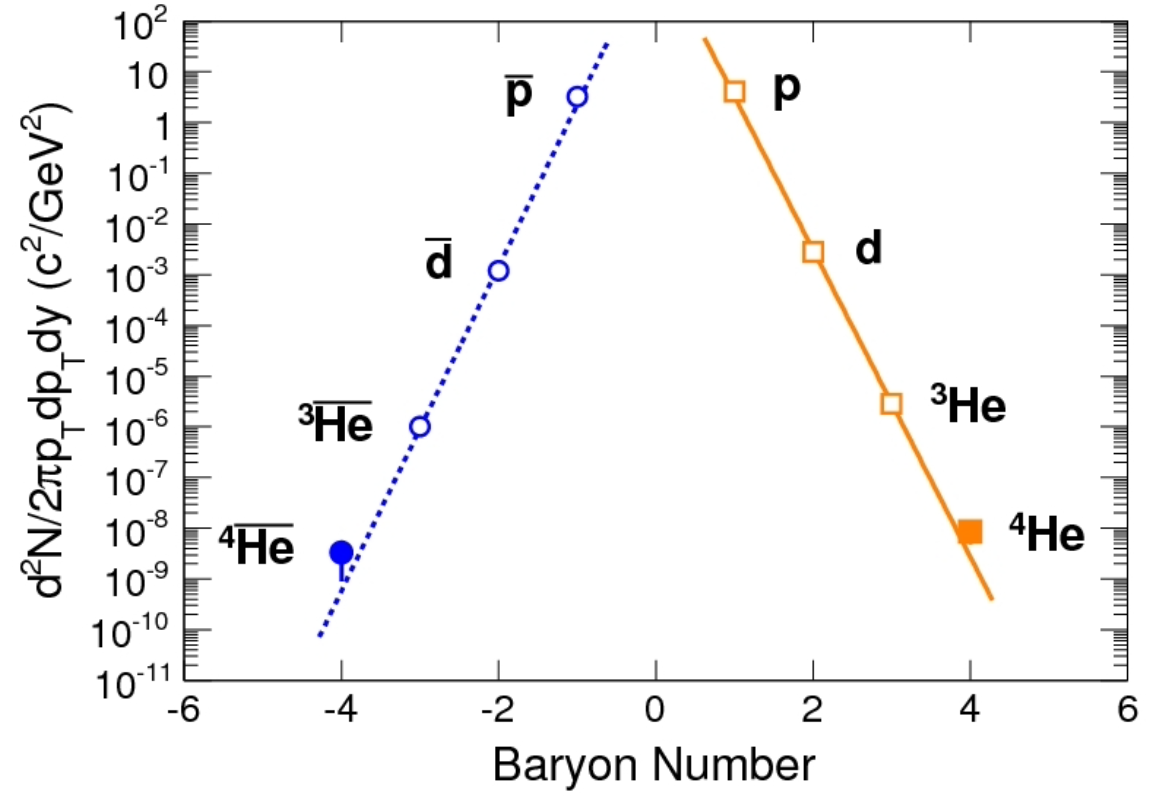
\includegraphics[width=0.4\textwidth]{Plots/He4Yield.png}
    \caption{\label{fig:He4Yield}不同核子数的产生指数率}
\end{figure}

\section{\label{sec:Sum}总结}
总而言之,QCD与QGP的复杂性需要相对论性重离子对撞实验的观测数据来指导模型的构建,因此位于BNL的RHIC和STAR成为了这一领域的焦点。STAR探测器的主体是他的时间投影室,因为时间投影室的优越性能,STAR可以在对带电粒子的径迹进行重构的同时,还能够对带电粒子进行很好的鉴别。这一点不仅仅对探测QGP事件末态的大量强子十分重要,还给人们探测反物质等提供了客观条件。同时,为了进一步提高STAR-TPC的分辨本领,考虑到STAR实验本身的需要,人们设计了基于多层电阻板室的飞行时间谱仪,这一谱仪加装后提高了STAR的探测本领,也使得一些新的分析得以开展。基于TPC的观测,人们发现了QGP的类液体性质,对QGP和QCD的认识有了一大步突破。此外,TPC,以及后续加装的ToF,也为反物质的探测提供了基础。

\bibliography{test.bib}
\end{document}
%
% ****** End of file apssamp.tex ******
